\documentclass[titlepage, letterpaper, 11pt]{article}
\usepackage[letterpaper, margin=1.25in]{geometry}
\usepackage{graphicx}
\usepackage{comment}
\usepackage{amsmath}
\usepackage{caption}
\usepackage{subcaption}
\usepackage{nicefrac}
\usepackage{tablefootnote}
\begin{document}

\title{Multi-Stage Tuned Amplifier}
\author{By: Ben Lorenzetti\\
Team Member: Francois Nyamsi}
\date{Project Start Date: January 22, 2015\\
Report Submission Date: February 8, 2015}
\maketitle

\clearpage
\mbox{}
\thispagestyle{empty}
\clearpage
\setcounter{page}{1}

\tableofcontents

\section{Objective}

To compare the operation of common-emitter and common-base tuned
amplifier stages, and to design and characterize a multi-stage,
high-gain IF amplifier for 10 MHz operation with 50$\Omega$ input and
output impedances.

\clearpage
\section{Principles of Operation}

Tuned amplifiers are critical for electronic communications because
they increase the power of desired signal but reject other frequencies
as noise. At 10 MHz, a tuned amplifier could be used with an antenna
to recieve HF amateur radio from the other side of the world
\footnote{10 MHz waves can traverse the curve of the earth because
they get reflected by charged particles in the ionosphere, called
ionospheric skip propagation.},
or could be used in a computer to recieve 10Base-T ethernet.

There are three possible circuit configurations for bipolar junction
transistors (BJT) biased in forward-active mode, based on
which terminals are used for input, output, and common reference.

\begin{figure}[ht]
	\centering
	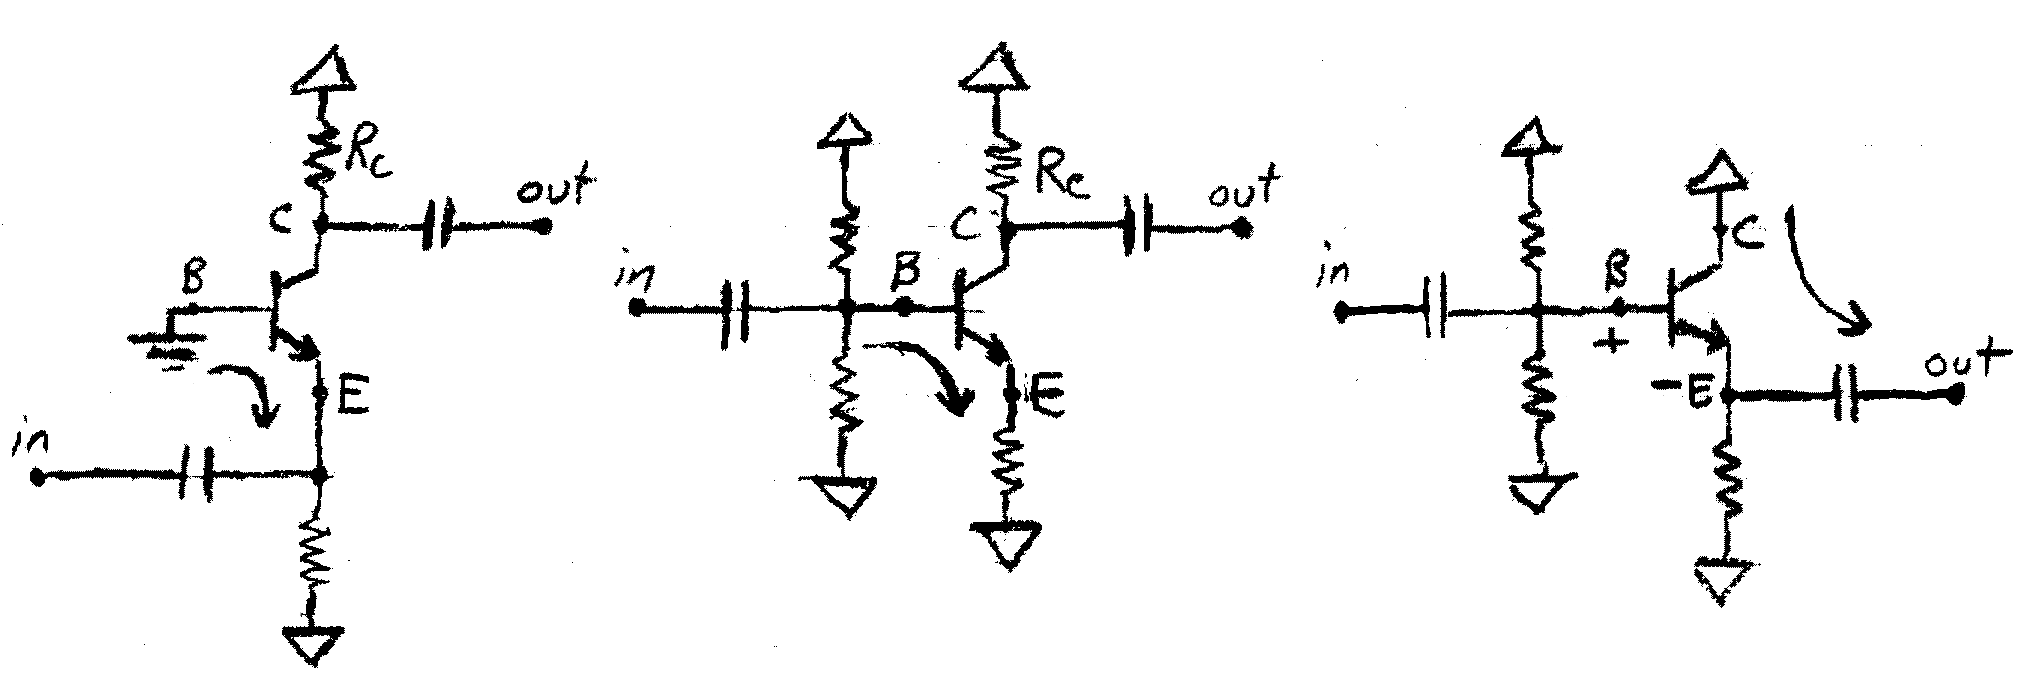
\includegraphics[width=0.75\textwidth]
		{figures/BJTforwardBiasConfigurations.png}
	\caption{
		Common-base (left), common-emitter (middle), and
		common-collector (right) configurations for BJT
		amplifiers.
	}
	\label{BJTforwardBiasConfigurations}
\end{figure}

Each configuration has its tradeoffs. The common-base (CB) configuration is
a good current buffer, with $A_{i}\approx1$ and low input impedance.
The common-emitter (CE) configuration offers the best overall power gain,
but $A_{v}$ and $A_{i}$ may vary with loadings. The common-collector
configuration is a good voltage buffer 
($A_{v}\approx1$) with low output impedance.

The three configurations can be cascaded together to gain the benefits
of each. If cascaded in the order shown in figure 
\ref{BJTforwardBiasConfigurations}, from left-to-right, the resulting
3-stage broadband amplifier would have low input impedance, good power
gain, and minimal output impedance.

A slight modification to the CE and CB configurations in figure
\ref{BJTforwardBiasConfigurations} can apply a filter to the broadband
amplifier; tuning the gain to a narrow frequency set by a tank circuit. 

Because BJTs are minority carrier devices, they act as current amplifiers
without being strongly affected by voltage. For the two configurations
where the output is at the collector (CB and CE), the BJT acts like a
dependent current source feeding the output load and the biasing
resistance $R_{C}$. As a result, the voltage gain for these
configurations is determined primarily by how difficult it is for
the collector current to reach ground; $A_{v}\propto R_{C}||R_{L}$.

One can take advantage of the collector current's obstinance
by replacing $R_{C}$ with an impedance that varies with frequency.
Using an inductor and a capacitor in parallel provides a short circuit
to ground for both DC and high frequency currents. Additionally, at the
LC circuit's resonant frequency, the net impedance $\rightarrow \infty$
due to power oscillating between the two.
\footnote{For this reason, an $L||C$ circuit is called a tank circuit.}
The result is a narrow bandpass filter at the resonant frequency, 
where $Z_{C}\rightarrow \infty$.

\section{Theory}

\subsection{Tank Circuits}

No inductor is ideal. The quality of an inductor is defined by
the ratio of the impedance and resistance of the discrete element.
\begin{equation*}
Q=\frac{X_{L}}{R_{S}}\qquad\textrm{where}\qquad Z_{L}=R_{S}+jX_{L}
\end{equation*}

The series resistance $R_{S}$ is due to the resistivity of the
wire and the length used to wrap the coil. Furthermore, the
impedance $X_{L}$ is not 100\% inductive; there is a distributed
capacitance $C_{D}$ between the surfaces of the tightly wrapped
wire. The circuit model for an inductor is shown in the left pane of
figure \ref{tankCircuit}.

As a consequence of the distributed capacitance, every inductor
will have a self resonant frequency $f_{0}$, at which the energy
entering the tank will oscillate between the inductor and capacitor
instead of passing through.

\begin{figure}[ht]
	\centering
	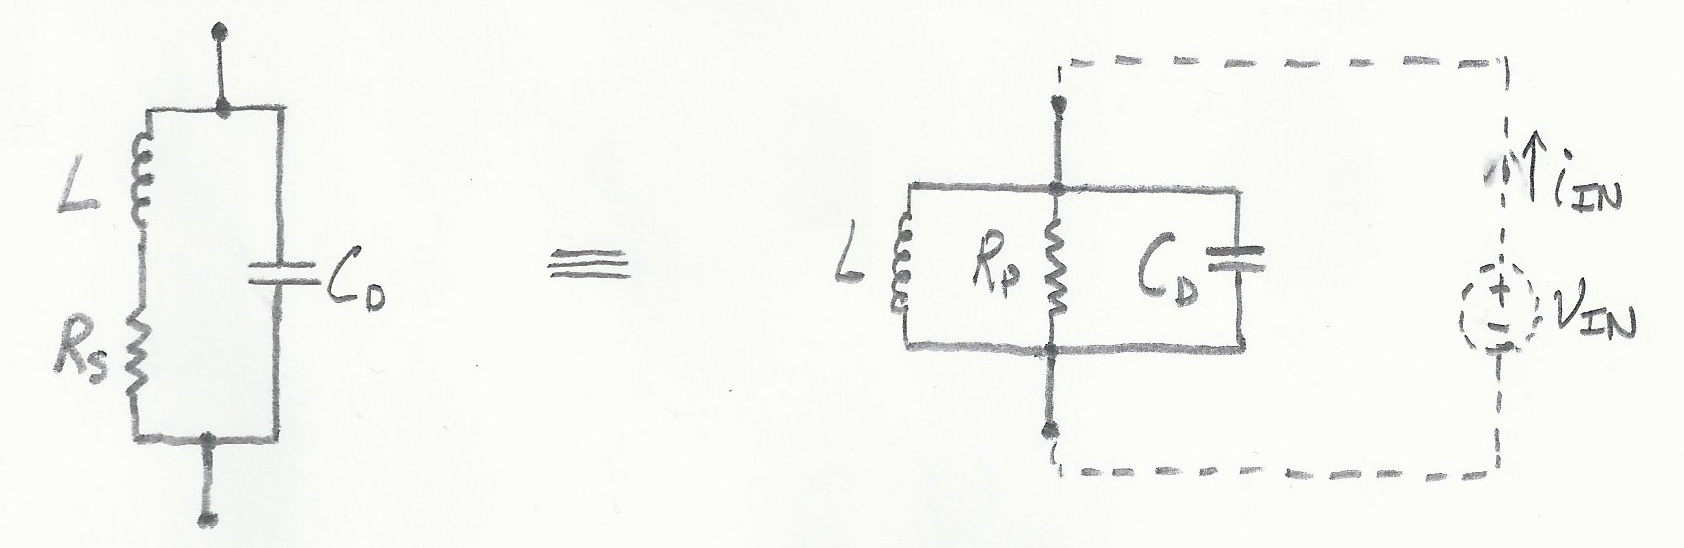
\includegraphics[width=0.75\textwidth]
		{figures/tankCircuit.png}
	\caption{
		Circuit model for a non-ideal inductor (left) and its
		parallel equivalent circuit (right).
	}
	\label{tankCircuit}
\end{figure}

Sometimes the parallel equivalent of the imperfect L model is more
convenient. If the quality is greater than 5 the conversion is easy:
\begin{equation}
Q=\frac{X_{L}}{R_{S}}=\frac{R_{P}}{X_{L}}
\end{equation}

The self resonance frequency occurs when the net impedance is
greatest. Applying Kirchoff's current law to the parallel model...

\begin{equation*}
|I_{in}|=\frac{|V_{in}|}
{\sqrt{(j\omega L+1/j\omega C)^{2}+R_{P}^{2}}}
\end{equation*}

\begin{equation}
|Z_{L}|=\sqrt{R_{P}^{2}-\left(\omega L-\frac{1}{\omega C}\right)^{2}}
\end{equation}

One can see that $Z_{L}$ will reach its peak when:
\begin{equation*}
\left(\omega L-\frac{1}{\omega C}\right)=0
\label{resonantFrequencyEq}
\end{equation*}

Therefore, the maximum impedance of a tank circuit is:
\begin{equation}
|Z_{L}|_{max}=R_{P}\qquad\textrm{when}\qquad
f_{0}=\frac{1}{2\pi\sqrt{LC}}
\end{equation}

More generally than non-ideal inductors; the resonant frequency,
bandwidth, and quality of a parallel RLC circuit are related to 
L, C, and R.
\begin{equation}
Q=\frac{\omega_{0}}{B}=\omega_{0}RC=\frac{R}{\omega_{0}L}
\label{parallelRLCequation}
\end{equation}

\subsection{Common-Base Broadband Amplifier}

The basic circuit for an single stage, common-base (CB) amplifier is
shown in figure \ref{commonBaseAmplifier}. The base terminal is
grounded and the input signal passes through the BJT from emitter
to collector. In this configuration, the BJT acts like a current
buffer, where the input current is repeated at the output regardless
of the load. 

\begin{figure}[ht]
	\centering
	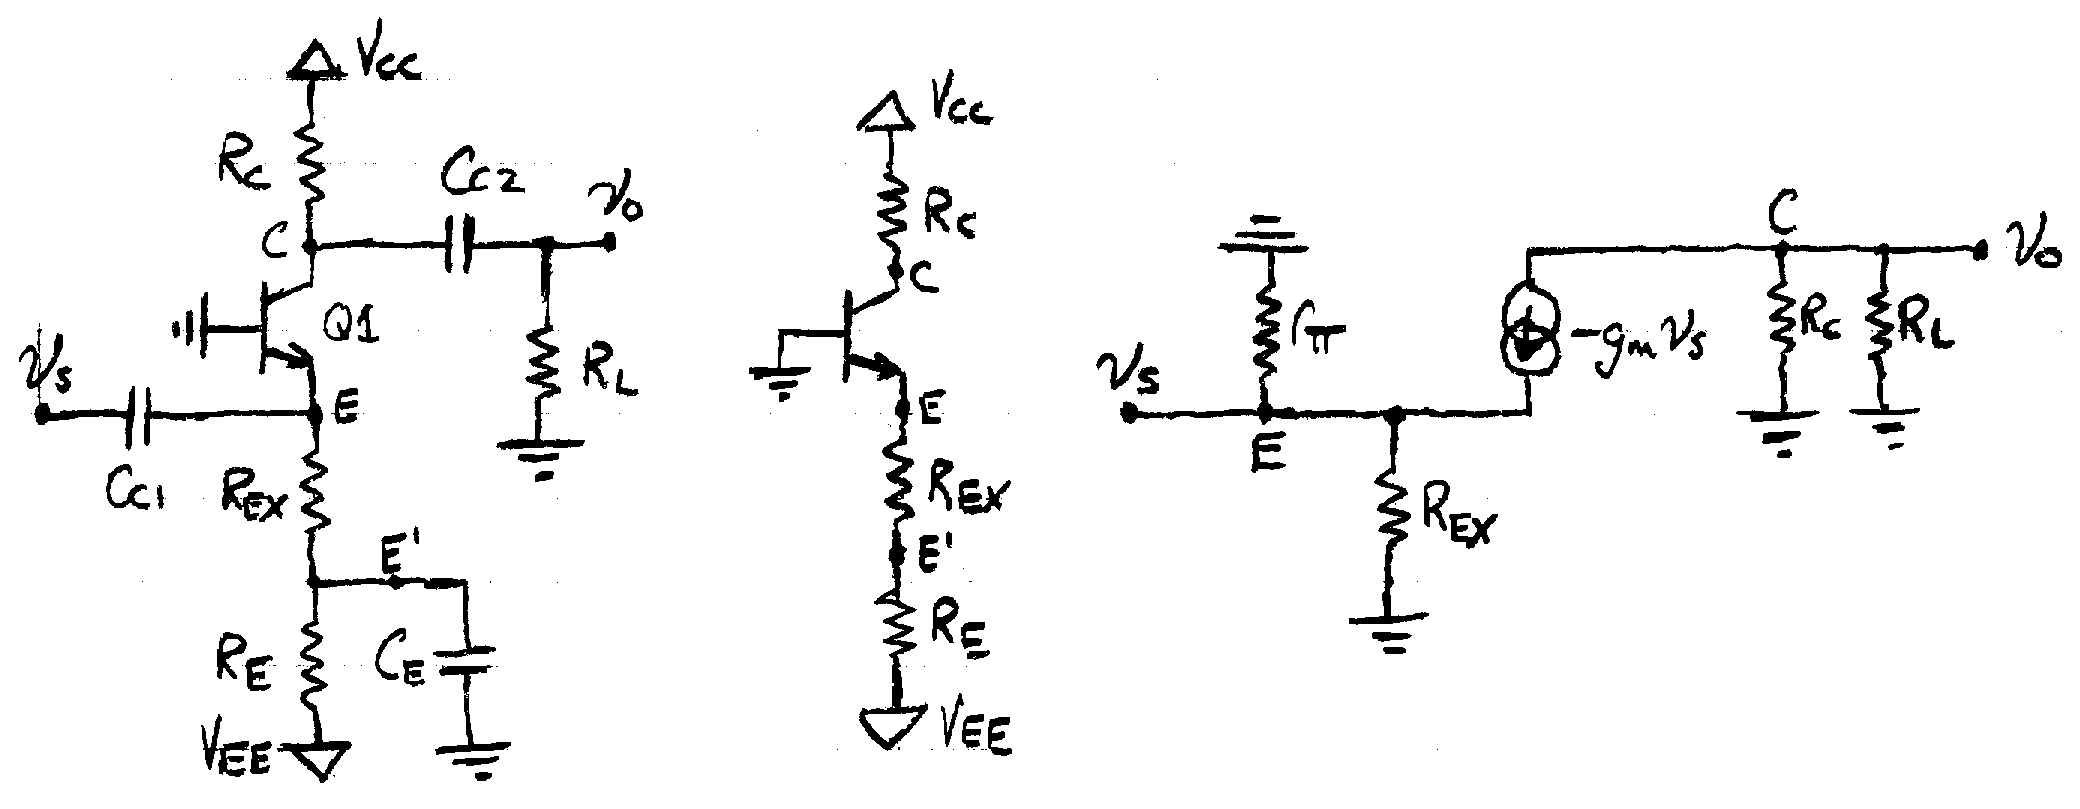
\includegraphics[width=\textwidth]
		{figures/commonBaseAmplifier.png}
	\caption{
		Basic circuit for a common-base broadband amplifier
		(left), its DC large signal (middle) equivalent, and
		AC small signal equivalent (right).
	}
	\label{commonBaseAmplifier}
\end{figure}

Two DC power rails are needed to bias the BJT in forward-active mode.
A positive supply holds the collector reverse biased
relative to the base which, at ground, is forward biased relative
to the negative supplied emitter. Quiescent point analysis of the
common-base is easy because the voltage is pinned at every node.

\begin{equation}
I_{EQ}=\frac{-V_{BE(on)}-V_{EE}}{R_{E}}
\label{cbIeq}
\end{equation}

\begin{equation}
r_{\pi}=\frac{V_{th}}{I_{BQ}}
=\frac{(\beta+1)V_{th}}{I_{EQ}}
\label{rPi}
\end{equation}

\begin{equation}
g_{m}=\frac{\beta}{r_{\pi}}
=\frac{\alpha I_{EQ}}{V_{th}}
\label{gm}
\end{equation}

The hybrid-$\pi$ model for small signal AC modeling is shown in the
right pane of figure \ref{commonBaseAmplifier}. Applying Kirchoff's
current law at node E can be used to find the input resistance.

\begin{equation*}
\textrm{KCL @ E:}\qquad
i_{S}-\frac{v_{s}}{r_{\pi}}-\frac{v_{s}}{R_{E}}-g_{m}v_{s}=0
\end{equation*}

\begin{equation*}
i_{s}=v_{s} \left[ \frac{1}{R_{\pi}}+\frac{1}{R_{E}}+g_{m} \right]
\end{equation*}

\begin{equation*}
i_{s}=v_{s} \left[
\frac{R_{E}+r_{\pi}+g_{m}r_{\pi}R_{E}}
{r_{\pi}R_{E}} \right]
\end{equation*}

\begin{equation*}
\frac{v_{s}}{i_{s}}
=\frac{r_{\pi}R_{E}}{R_{E}+r_{\pi}+g_{m}r_{\pi}R_{E}}
\end{equation*}

\begin{equation*}
R_{in}=\frac{r_{\pi}}{\beta+1+\frac{r_{\pi}}{r_{E}}}
\end{equation*}

\begin{equation}
R_{in}=\frac{r_{\pi}}{\beta+1}
\left[\frac{1}{1+\nicefrac{r_{\pi}}{(\beta+1)R_{E}}}\right]
\label{commonBaseRin}
\end{equation}

Applying KCL at the collector can be used to calculate the voltage
gain of a single common-base stage.

\begin{equation*}
\textrm{KCL @ C:}\qquad
g_{m}v_{s}+\frac{v_{o}}{R_{L}}+\frac{v_{o}}{R_{C}}=0
\end{equation*}

\begin{equation*}
v_{o}\left[\frac{R_{L}+R_{C}}{R_{L}R_{C}}\right]=g_{m}v_{s}
\end{equation*}

\begin{equation}
A_{v}=\frac{g_{m}R_{L}R_{C}}{R_{L}+R_{C}}
\label{cbAv}
\end{equation}

\subsection{Common-Emitter Broadband Amplifier}

The basic circuit for an single stage, common-emitter (CE)
amplifier is shown in figure \ref{commonEmitterAmplifier}.
The DC equivalent circuit is shown in the left pane of figure
\ref{commonEmitterEquivalentCircuits}; the AC in the right.

\begin{figure}[ht]
	\centering
	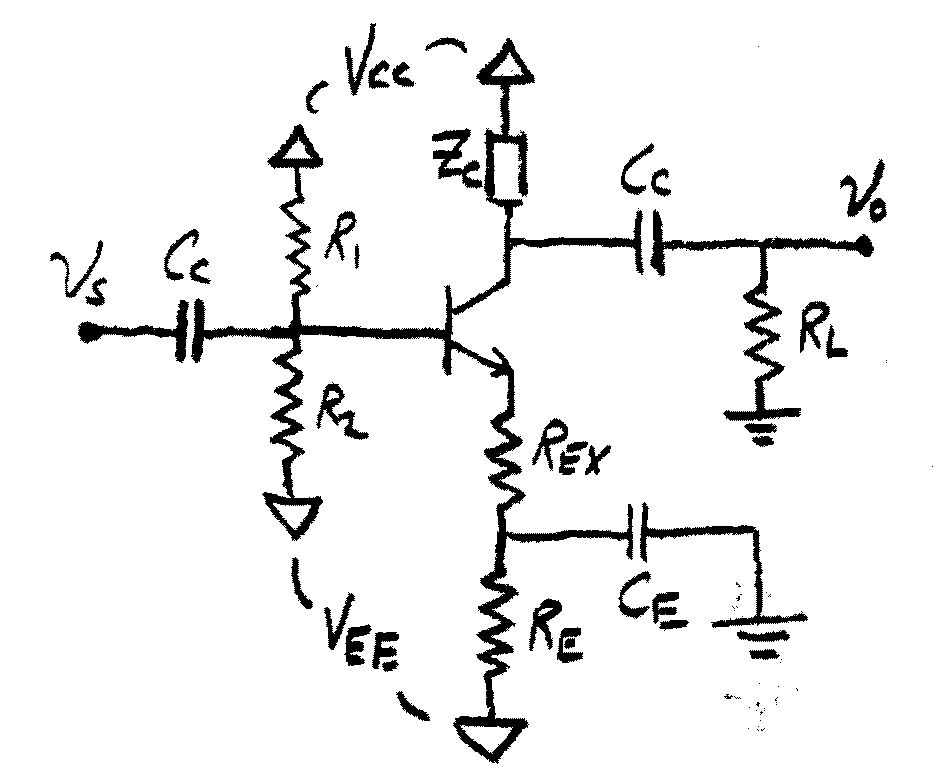
\includegraphics[width=0.35\textwidth]
		{figures/commonEmitterAmplifier.png}
	\caption{
		Broadband Common-Emitter Stage
	}
	\label{commonEmitterAmplifier}
\end{figure}

\begin{figure}[ht]
	\centering
	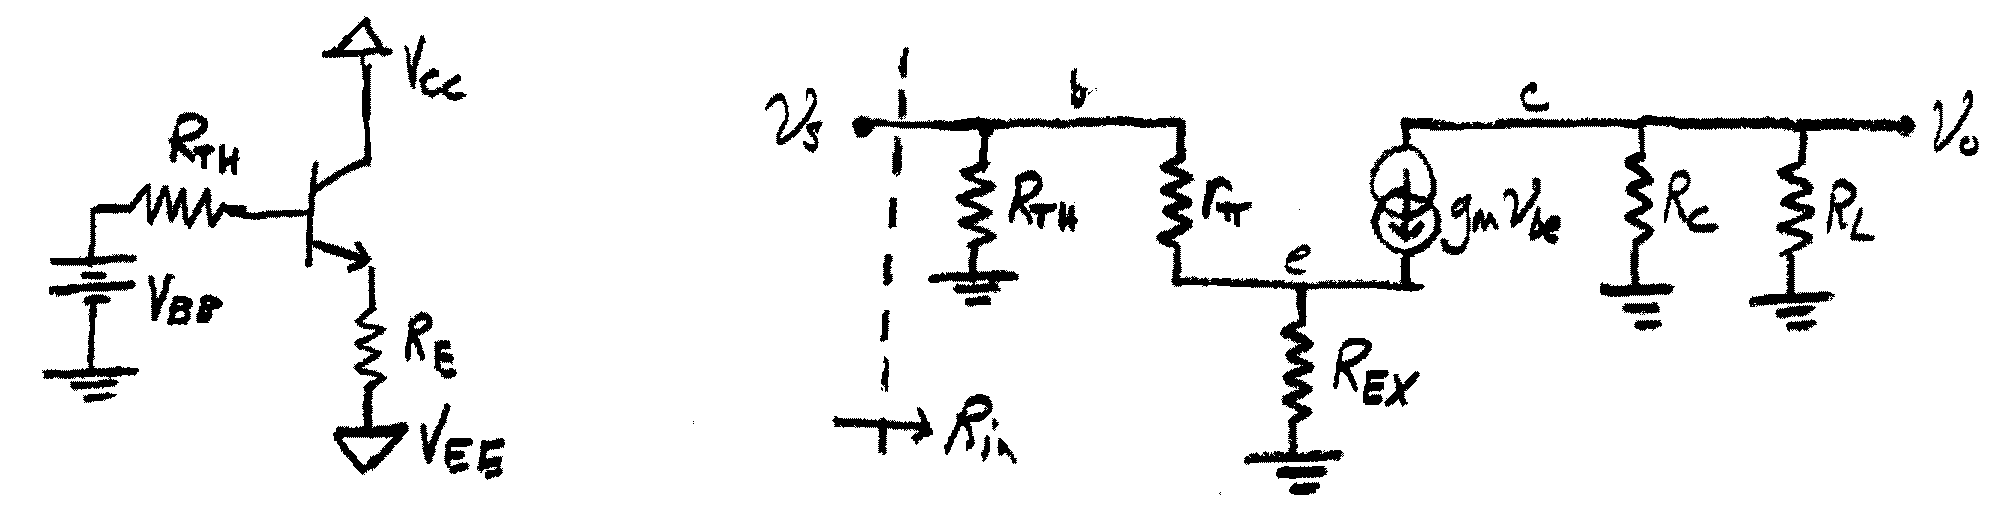
\includegraphics[width=0.8\textwidth]
		{figures/commonEmitterEquivalentCircuits}
	\caption{
		Common-emitter equivalent circuits: DC (left),
		AC (right).
	}
	\label{commonEmitterEquivalentCircuits}
\end{figure}

The DC equivalent circuit, shown in figure
\ref{commonEmitterEquivalentCircuits}, used a thevenin source
conversion from the base bias resistors $R_{1}$ and $R_{2}$. The
thevenin equivalent's parameters are found by
\begin{equation}
R_{TH}=R_{1}||R_{2}=\frac{R_{1}R_{2}}{R_{1}+R_{2}}
\end{equation}
and
\begin{equation}
V_{BB}=V_{EE}+\frac{R_{2}}{R_{1}+R_{2}}(V_{CC}-V_{EE})
\end{equation}

The same thevenin conversion was used for the AC circuit in figure
\ref{commonEmitterEquivalentCircuits} for $R_{TH}$. The other
parameters in the AC equivalent circuit come from the hybrid-$\pi$
model, defined previously in equations \ref{rPi} and \ref{gm}.

The DC loading characteristics are easily found by using KVL on the
collector-emitter loop.

\begin{equation*}
V_{CC}-V_{CE}-R_{E}I_{EQ}-V_{EE}=0
\end{equation*}

\begin{equation}
I_{E}=\frac{V_{CC}-V_{EE}}{R_{E}}-\frac{V_{CE}}{R_{E}}
\label{ceDCloadEquation}
\end{equation}

The AC characteristics require a little more algebra. We are
interested in the small signal voltage gain and input resistance
for a CE stage. Kirchoff's current law at the emitter node of the 
AC equivalent circuit (figure \ref{commonEmitterEquivalentCircuits},
right pane) can be written:
\begin{equation*}
\frac{v_{e}-v_{s}}{r_{\pi}}+\frac{v_{e}}{R_{EX}}+g_{m}(v_{e}-v_{s})=0
\end{equation*}

Collecting terms and separating variables gives:
\begin{equation*}
v_{e}\left[\frac{1}{r_{\pi}}+\frac{1}{R_{EX}}+g_{m}\right]
=v_{s}\left[\frac{1}{r_{\pi}}+g_{m}\right]
\end{equation*}

Multiplying both sides by $r_{\pi}$ and $R_{EX}$ gives:
\begin{equation*}
v_{e}[R_{EX}(1+\beta)+r_{\pi}]=v_{s}(1+\beta)R_{EX}
\end{equation*}

So the ratio between $v{e}$ and $v_{s}$ is:
\begin{equation*}
\frac{v_{e}}{v_{s}}=
\left[\frac{(1+\beta)R_{EX}}{(1+\beta)R_{EX}+r_{\pi}}\right]
\end{equation*}

Looking ahead, in the interest of saving paper, it would be better
to have an expression for $v_{s}-v_{e}$ as a function of $v_{s}$.
\begin{equation*}
v_{s}-v_{e}=
v_{s}\left[1-\frac{v_{e}}{v_{s}}\right]=
v_{s}\left[1-\frac{(1+\beta)R_{EX}}{(1+\beta)R_{EX}+r_{\pi}}\right]
\end{equation*}

\begin{equation}
v_{s}-v_{e}=
\left[\frac{r_{\pi}}{(1+\beta)R_{EX}+r_{\pi}}\right]v_{s}
\label{vsMinusVe}
\end{equation}

The small signal voltage gain can be found from Ohm's law, applied
across the resistors between the output and ground.
\begin{equation*}
v_{o}=(R_{C}||R_{L})*g_{m}(v_{s}-v_{e})
\end{equation*}

Substituting equation \ref{vsMinusVe} for the voltage difference and
then recognizing that $r_{\pi}g_{m}=\beta$...
\begin{equation*}
v_{o}=(R_{C}||R_{L})
\left[\frac{\beta}{(1+\beta)R_{EX}+r_{\pi}}\right]v_{s}
\end{equation*}

Dividing both sides by $v_{s}$ and pulling $\alpha$ out of the
bracket gives us the magnitude of the transfer function in generic
form.
\begin{equation}
A_{v(CE)}=\frac{(R_{C}||R_{L})}{R_{EX}}*\frac{\beta}{\beta+1}*
\frac{1}{1+\nicefrac{r_{\pi}}{(\beta+1)R_{EX}}}
\label{ceAv}
\end{equation}

Now for the small-signal input resistance; the ratio between
$v_{s}$ and $i_{s}$ in for the AC equivalent circuit in figure
\ref{commonEmitterEquivalentCircuits}. Writing KCL at the base node
yields
\begin{equation*}
-i_{s}+\frac{v_{s}}{R_{TH}}+\frac{v_{s}-v_{e}}{r_{\pi}}=0
\end{equation*}

Substituting equation \ref{vsMinusVe} for $v_{s-e}$ 
eliminates $v_{e}$
\begin{equation*}
i_{s}=\frac{v_{s}}{R_{TH}}+\frac{v_{s}}{r_{\pi}}
\left[\frac{r_{\pi}}{(1+\beta)R_{EX}+r_{\pi}}\right]
\end{equation*}

Dividing both sides by $v_{s}$ gives the input conductance,
but the partial fractions must be prepared for inversion.
\begin{equation*}
G_{in}=
\left[\frac{1}{R_{TH}}+\frac{1}{(1+\beta)R_{EX}+r_{\pi}}\right]=
\left[\frac{(1+\beta)R_{EX}+r_{\pi}+R_{TH}}
{R_{TH}(R_{EX}(1+\beta)+r_{\pi})}\right]
\end{equation*}

Inverting the conductance and pulling
$(1+\beta)R_{EX}+r_{\pi}$ out of both numerator and denominator gives
the input resistance in generic form.
\begin{equation*}
R_{in}=R_{TH}
\left[\frac{1}{1+\nicefrac{R_{TH}}{(1+\beta)R_{EX}+r_{\pi}}}\right]
\end{equation*}

If one assumes that $R_{TH}>>(1+\beta)R_{EX}+r_{\pi}$, then the
$+1$ term in the denominator is negligible and the input resistance
simplifies to
\begin{equation}
R_{in(CE)}=(1+\beta)R_{EX}+r_{\pi}
\label{ceRin}
\end{equation}

\subsection{Common-Collector Broadband Amplifier}

When the BJT is configured such that the collector is common to both
input and output, the amplifier acts like a voltage buffer; providing
current gain as necessary and having low output impedance. The
common-collector circuit is shown in figure
\ref{commonCollectorAmplifier}. The right pane is the AC equivalent
circuit. The DC equivalent circuit is identical to that of the CE
amplifier, shown in the left pane of figure
\ref{commonEmitterEquivalentCircuits}.

\begin{figure}[ht]
	\centering
	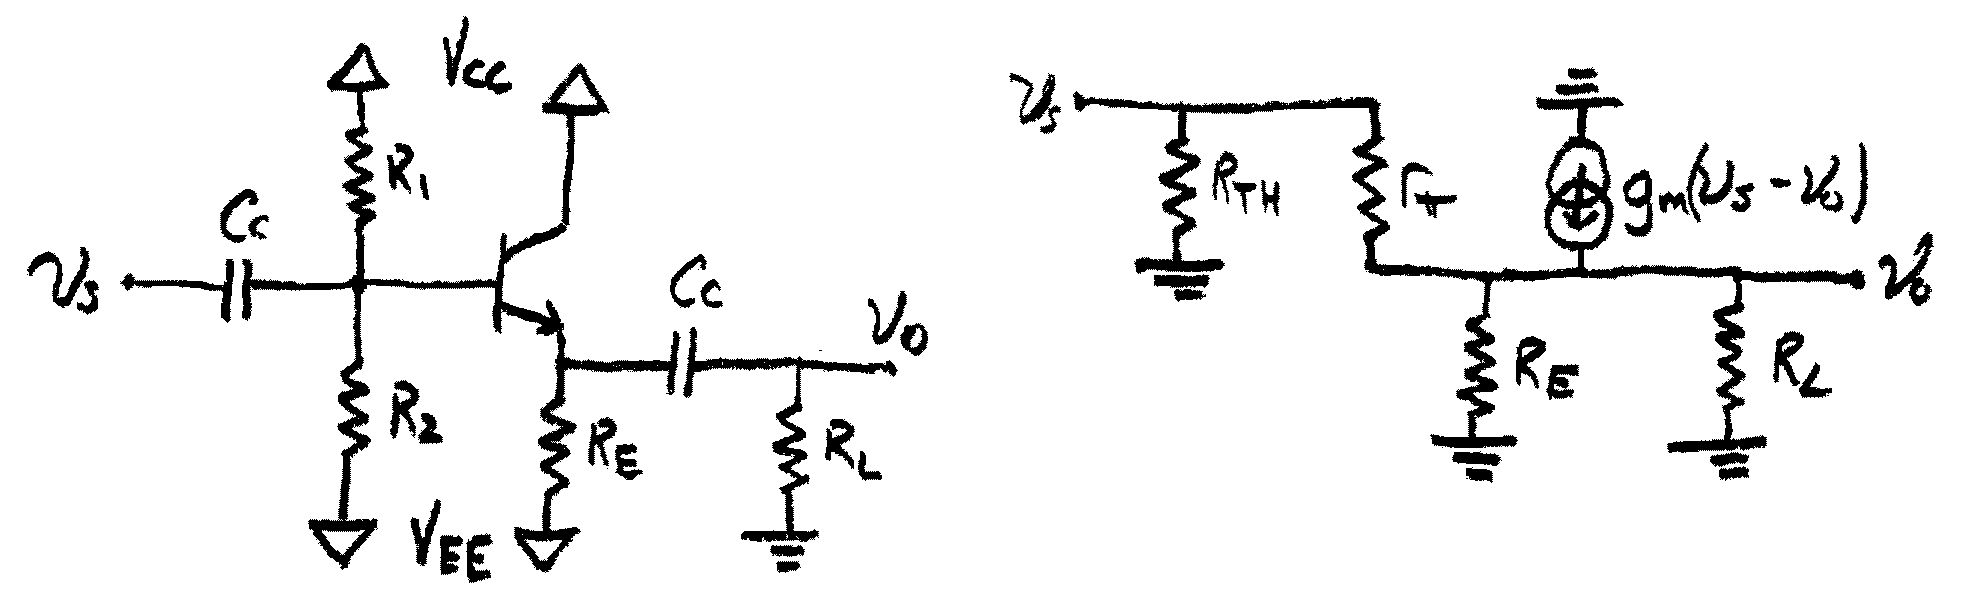
\includegraphics[width=.75\textwidth]
		{figures/commonCollectorAmplifier.png}
	\caption{
		Basic circuit for a common-collector broadband amplifier
		(left) and its AC equivalent circuit (right).
	}
	\label{commonCollectorAmplifier}
\end{figure}

The small-signal voltage gain should be close to unity, but this can
be shown by taking KCL at the emitter node in the AC model in figure
\ref{commonCollectorAmplifier}.
\begin{equation*}
\frac{v_{o}-v_{s}}{r_{\pi}}+\frac{v_{o}}{R_{E}}+\frac{v_{o}}{R_{L}}
-g_{m}(v_{s}-v_{o})=0
\end{equation*}

Multiplying through by $r_{\pi}$ and separating variables cleans this
up somewhat,
\begin{equation*}
v_{o}\left[1+\beta+\frac{r_{\pi}}{R_{E}}+\frac{r_{\pi}}{R_{L}}\right]
=v_{s}[1+\beta]
\end{equation*}

The coefficients must be prepared for inversion.
\begin{equation*}
v_{o}\left[\frac{(1+\beta)R_{E}R_{L}+r_{\pi}(R_{E}+R_{L})}
{R_{E}R_{L}}\right]=
v_{s}[1+\beta]
\end{equation*}

So the voltage gain of the common-collector is
\begin{equation*}
A_{v}=\frac{(1+\beta)R_{E}R_{L}}
{(1+\beta)R_{E}R_{L}+r_{\pi}(R_{E}+R_{L})}
\end{equation*}

This can be rewritten in generic transfer form.
\begin{equation}
A_{v(CC)}=\frac{1}{1+\nicefrac{r_{\pi}}{(1+\beta)(R_{E}||R_{L})}}
\label{ccAv}
\end{equation}

The voltage gain is observed to be $\nicefrac{1}{2}$ when the load
resistance is equal to the output impedance. This is the case if the
ratio term in the generic form equation is unity. Mathematically,
this is expressed as
\begin{equation*}
\frac{r_{\pi}}{(\beta+1)(R_{E}||R_{o})}=1
\end{equation*}

Substituting equation \ref{rPi} in place of $r_{\pi}$ and assuming
that $R_{E}>>R_{o}$ yields a surprisingly simple equation for output
impedance.
\begin{equation}
R_{o(CC)}=\frac{V_{thermal}}{I_{EQ}}
\label{ccRo}
\end{equation}

\subsection{Voltage Gain and $I_{EQ}$}
\label{gainVSquiescentCurrent}

Substituting equation \ref{gm} for $g_{m}$ into equation \ref{cbAv}
gives voltage gain of a CB amplifier as a function of quiescent
current. Similaryly, substituting equation \ref{rPi} for $r_{\pi}$
into equation \ref{ceAv} gives the small-signal gain of a CE
amplifier.
\begin{equation}
A_{v(CB)}=\frac{\alpha(R_{L}||R_{C})I_{EQ}}{V_{th}}
\end{equation}

\begin{equation}
A_{v(CE)}=\frac{\alpha(R_{C}||R_{L})}{R_{EX}}
\left[\frac{1}{1+\nicefrac{V_{th}}{R_{EX}I_{EQ}}}\right]
\end{equation}

Using typical resistor values, the small-signal gain of broadband
common-base and common-emitter amplifiers was plotted as a function
of DC biasing. The MATLAB script used to generate plot
\ref{gainQptRelation} is included in appendix \ref{matlabScript}.

\begin{figure}[ht]
	\centering
\begin{comment}
	\includegraphics[width=0.5\textwidth]
		{figures/gainQptRelation}
\end{comment}
	\caption{
		Relationship Between AC Voltage Gain and DC Biasing
		for CB and CE Amplifier
	}
	\label{gainQptRelation}
\end{figure}


\subsection{Coupling Capacitors}

The coupling capacitors, labeled $C_{Cx}$, isolate each stage from
direct currents but provide a low impedance path for the AC signal.
Taken together, they should form a sharp high-pass filter with its
corner frequency below 1000 Hz. The 3dB corner occurs when half the
signal power is dissipated in the capacitor and half in the stage's
input. This occurs when $Z_{Cc}=Z_{in}$.

\begin{equation*}
\frac{1}{|j\omega C|}=R_{in}
\end{equation*}

\begin{equation}
C_{C}\geq \frac{159.15\,\mu F*\Omega}{R_{in}}
\label{couplingCapacitors}
\end{equation}

\section{Design and Simulation}

\subsection{Specifications}

The multi-stage amplifier must meet the following specifications in
table \ref{labSpecs}.

\begin{table}[ht]
\centering
\caption{Lab Specifications}
\begin{tabular}{l c c}
\hline
power supply			&$\pm 12V$	\\
passband center frequency	&$10MHz$	\\
bandwidth			&$300kHz$	\\
input impedance			&$50\Omega$	\\
ouptut impedance		&$50\Omega$	\\
gain at center frequency	&$>60dB$	\\
\hline
\end{tabular}
\label{labSpecs}
\end{table}

\subsection{BJT Characterization}

Four npn 2N2904 BJTs were characterized using the Tektronix curve
tracer and an HP LCR meter. The results are shown in table
\ref{BJTcharacteristics}. The current amplification factors ($\beta$
or $h_{fe}$) were taken with DC biasing close to their designed use;
the actual $I_{C}-V_{CE}$ characteristic curves appear later,
as the DC design is described.

\begin{table}[ht]
\centering
\caption{Measured BJT Characteristics}
\begin{tabular}{c|c|c|c|c}
\hline\hline
	&Q1	&Q2	&Q3	&Q4	\\
\hline\hline
$\beta$	&181	&191	&189	&189	\\
$V_{A}$	&260V	&273V	&273V	&224V	\\
$C_{CB}$\tablefootnote{measurement taken at $10MHz$}	&5.1pF	&5.19pF	&5.18pF	&5.23pF	\\
$C_{BE}$&3.26pF	&3.28pF	&3.30pF	&3.24pF	\\ 
\hline\hline
\end{tabular}
\label{BJTcharacteristics}
\end{table}

\subsection{Tank Circuit Characterization}

Two inductors were wound with \char`\~22 turns. Their inductance and quality
were measured using a Hewlett-Packard 4342A Q Meter. An appropriate
discrete capacitor and trimming capacitor were selected for both to
obtain a tank circuit with resonance at ~10 MHz. The fixed capacitors
were soldered to their inductors in parallel.

The soldered LC circuit were breadboarded in parallel with a trimming
capacitor and tuned. Then, the breadboarded tank circuit was measured
for net capacitance, resonance frequency, and quality using the HP
Q Meter. The methods for these measurements are attached in appendix
\ref{qMeter} and the results are shown in table
\ref{tankCircuitCharacteristics}.

\begin{table}[ht]
\centering
\caption{Tank Circuit Design and Measured Characteristics}
\begin{tabular}{c|c|c|c|c}
\hline\hline
Parameter	&1		&2		&3		&Description	\\
\hline\hline
$L$		&$3.0\mu H$	&$4.2\mu H$	&$4.4\mu H$	&measured inductor	\\
$Q_{L}$		&250		&90		&65		&on HP Q Meter	\\
\hline
$C_{target}$	&84.0pF		&60.3pF		&57.6pF		&from eq. \ref{resonantFrequencyEq}	\\
$C_{fixed}$	&55.6pF		&33pF		&34.1pF		&nominal value		\\
$C_{trim}$	&27.2pF		&31pF		&30.1pF		&approx		\\
\hline
$C_{d}$		&80pF		&61.7pF		&64.3pF		&measured LC circuit	\\
$f_{0}$		&12.8MHz	&13.9MHz	&13.8MHz	&on HP Q Meter,		\\
$Q$		&90		&110		&80	&see \ref{qMeter}	\\
$R_{p}$		&$21.7k\Omega$	&$40.3k\Omega$	&$30.4k\Omega$	&from eq. \ref{parallelRLCequation}	\\
\hline\hline
\end{tabular}
\label{tankCircuitCharacteristics}
\end{table}

\subsection{Common-Base Stage I}

The first stage must be a common-base amplifier in order to achieve
low input resistance. The emitter resitance must be
chosen to achieve desirable input resistance and voltage gain.

\begin{figure}[ht]
	\centering
	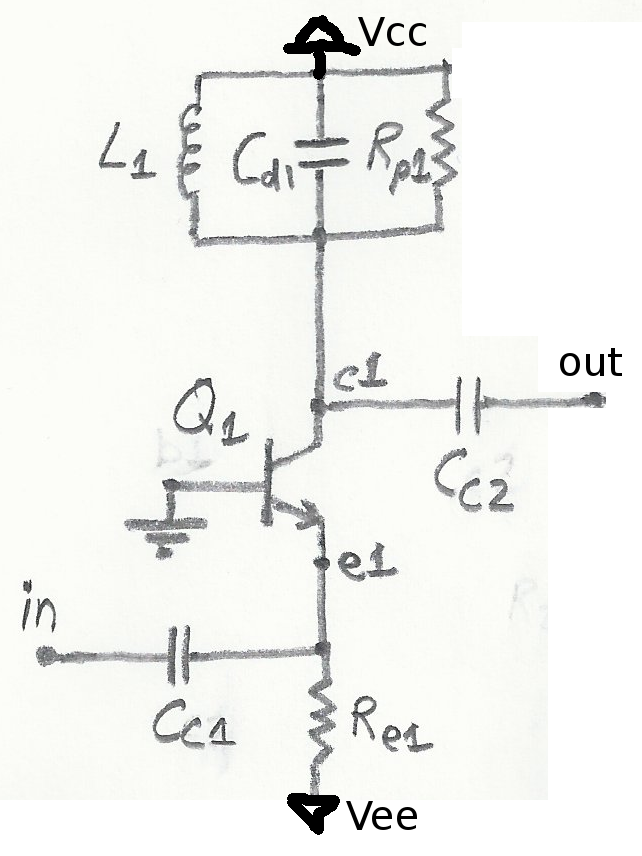
\includegraphics[width=0.23\textwidth]
		{figures/commonBaseStage}
	\caption{
		Common-base stage with SPICE netlist labels.
	}
	\label{commonBaseStage}
\end{figure}


It is clear that $R_{in}$ is strongly related to $r_{\pi}$ from
equation \ref{commonBaseRin}. If one assumes that
$r_{\pi}<<(\beta+1)R_{E}$, then the generic form fraction becomes one
and the input resistance becomes
\begin{equation*}
R_{in}|_{\nicefrac{r_{\pi}}{(\beta+1)R_{E}}\rightarrow 0}
=\frac{r_{\pi}}{\beta+1}
\end{equation*}

The value of $r_{\pi}$ varies depending on the quiescent operating
point. To achieve an input resistance of $50\Omega$, the quiescent
current $I_{EQ}$ must be chosen such that $r_{\pi}/\beta+1$ is 50.
Luckily it is easy to design $I_{EQ}$ for the CB stage; equation
\ref{cbIeq} shows that is is determined by $R_{E}$. Substituting
equations \ref{rPi} and \ref{cbIeq} into the expression for $R_{in}$
gives
\begin{equation*}
R_{in}=\frac{(\beta+1)V_{th}}{(\beta+1)I_{EQ}}=
\frac{V_{th}}{I_{EQ}}=
\frac{V_{th}}{-V_{BE(on)}-V_{EE}}R_{E}
\end{equation*}

By solving this expression, the designed value for $R_{E1}$ is
\begin{equation*}
R_{E1}=\frac{-0.7V+12V}{0.0259V}*50\Omega=21.814\,k\Omega
\end{equation*}

With $R_{E}$, the quiescent current is known from equation
\ref{cbIeq}; $I_{EQ}=0.52mA$. Armed with this knowledge, the first
BJT was characterized and a DC load line drawn. Because all of the
node voltages are pinned, the load line is vertical; $V_{CE}$ is 
independent of $I_{EQ}$.

\begin{figure}[ht]
	\centering
	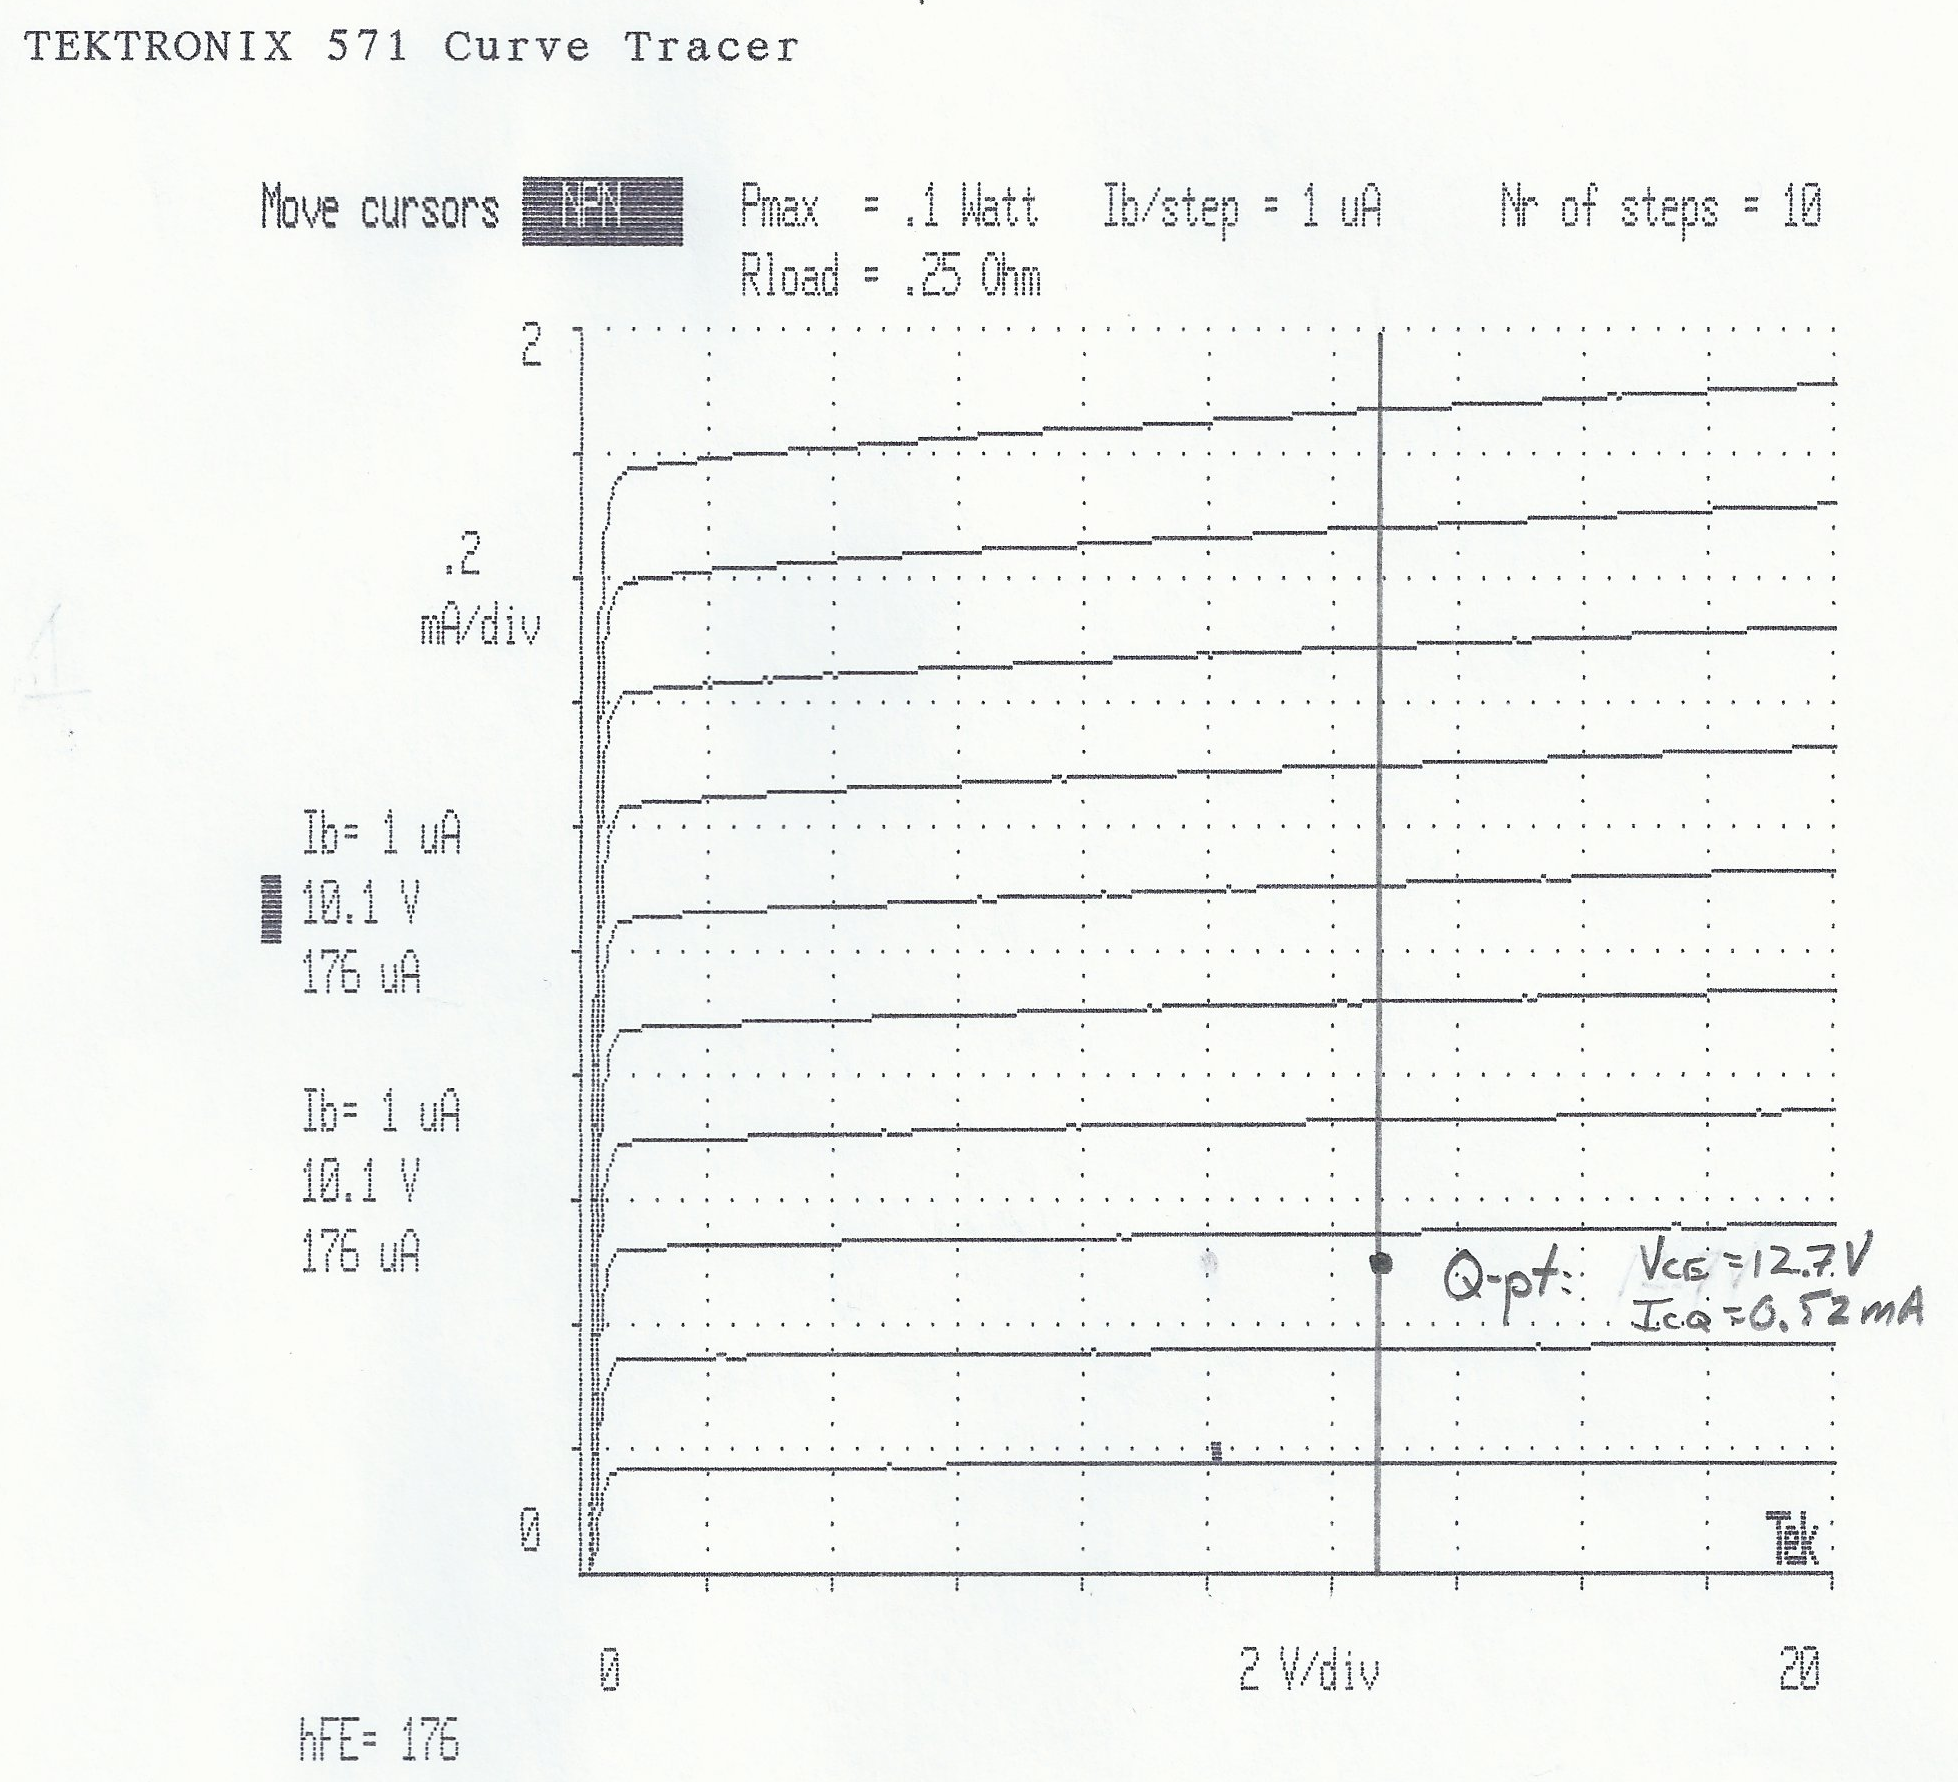
\includegraphics[width=0.6\textwidth]
		{measurements/q1Characteristics}
	\caption{
		Q1 Current-Voltage Characteristics and DC Load Line
	}
	\label{q1Characteristics}
\end{figure}

From equation \ref{couplingCapacitors} and using $R_{in}=50\Omega$,

\begin{equation*}
C_{C1}\geq 3.183pF
\end{equation*}

At this point, all of the discrete components for the CB stage have
been determined. A SPICE simulation was performed to check the
performance of the stage. For a load value, the input resistance of
the first common emitter stage was used. The netlist used is included
in appendix \ref{CBstageNetlist} and the results are shown in figure
\ref{CBstageMagnitudePlot}.

\begin{figure}[ht]
	\centering
	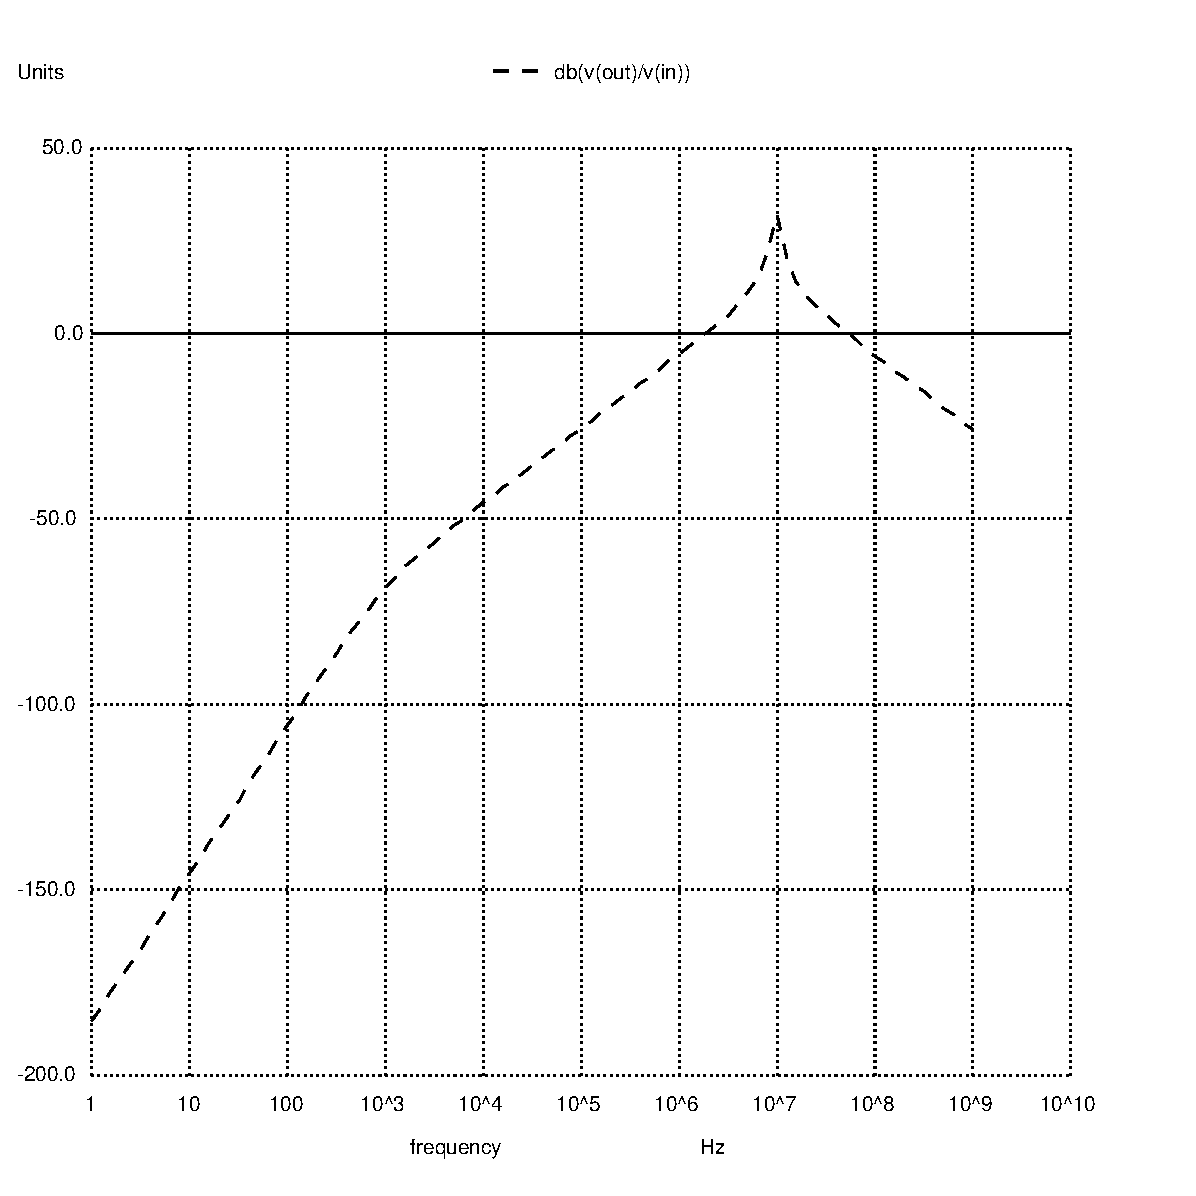
\includegraphics[width=0.5\textwidth]
		{ngspice/CBstage.eps}
	\caption{
		Magnitude Gain of Common-Base Stage, in dB
	}
	\label{CBstageMagnitudePlot}
\end{figure}

The CB stage was assembled on the breadboard and tested for its
frequency response. A load resistor of $12.5k\Omega$ was included.
The results are shown in figure \ref{CBstageMagnitudePlot}.

\subsection{Common-Emitter Stage II}
\label{stage2section}

The common-emitter configuration provides the highest overall power
gain, compared to CB and CC. This makes it ideal for the middle
stages. A single CE stage is shown in figure 
\ref{commonEmitterStage}.

\begin{figure}[ht]
	\centering
	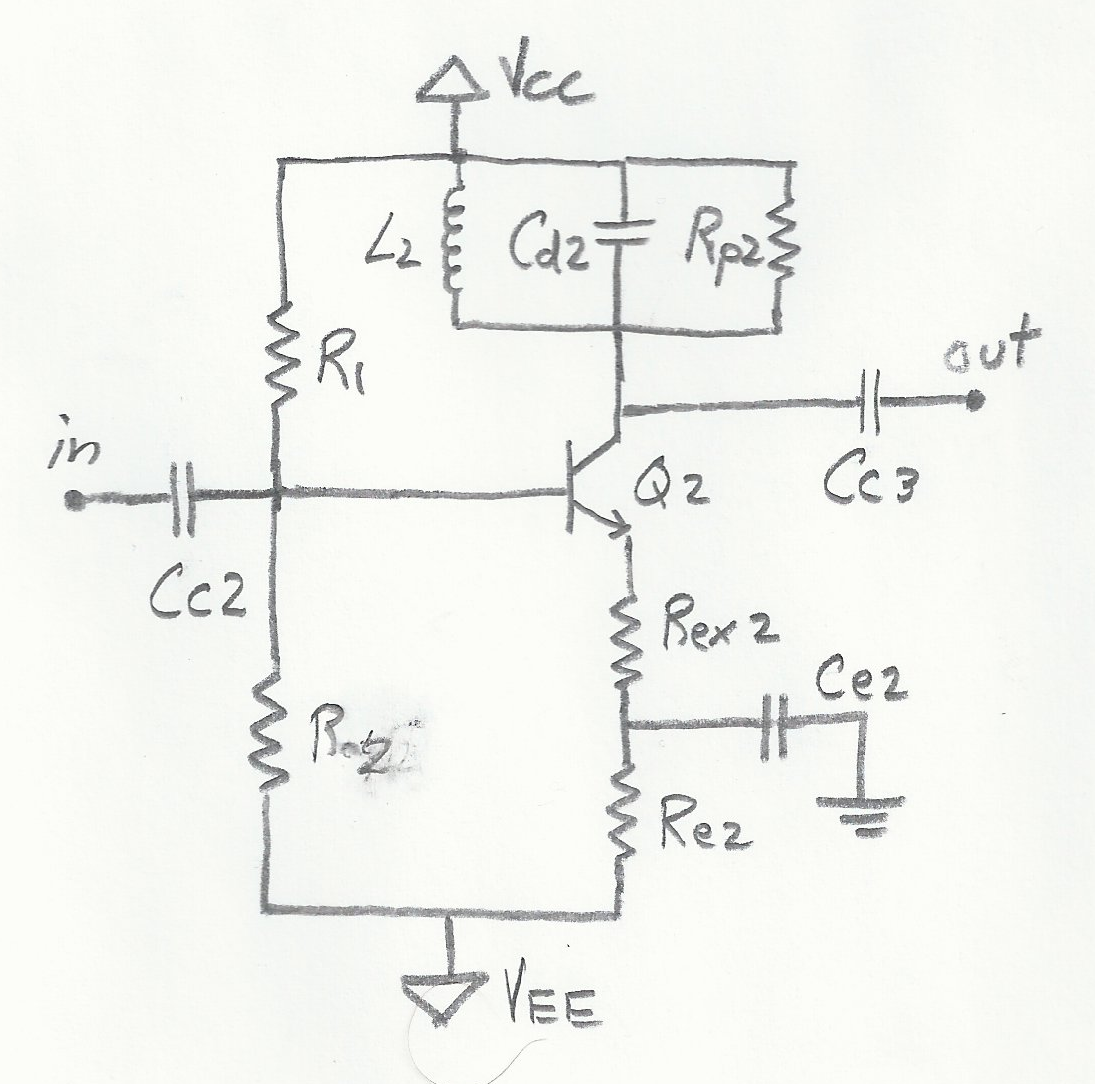
\includegraphics[width=0.35\textwidth]
		{figures/commonEmitterStage}
	\caption{
		Common-emitter stage with SPICE netlist labels.
	}
	\label{commonEmitterStage}
\end{figure}

The MATLAB analysis of $A_{v}(I_{EQ})$ in section
\ref{gainVSquiescentCurrent} showed that the gain of a CE amplifier
grows with increasing quiescent current up to a certain point. Based
on this, $I_{EQ}$ was designed to be near 1 mA.

The exact value for $I_{EQ}$ was chosen based on the closest curser
position to 1 mA when the BJT was characterized on the Tektronix
curve tracer. To allow for maximum swing between the $\pm12V$ rails,
$V_{EQ}$ was chosen to be 12 V. The I-V characteristics and DC load
line are shown in figure \ref{q2Characteristics}. The load line was
drawn using the chosen Q-pt and a cutoff of 24 V.

\begin{figure}[ht]
	\centering
	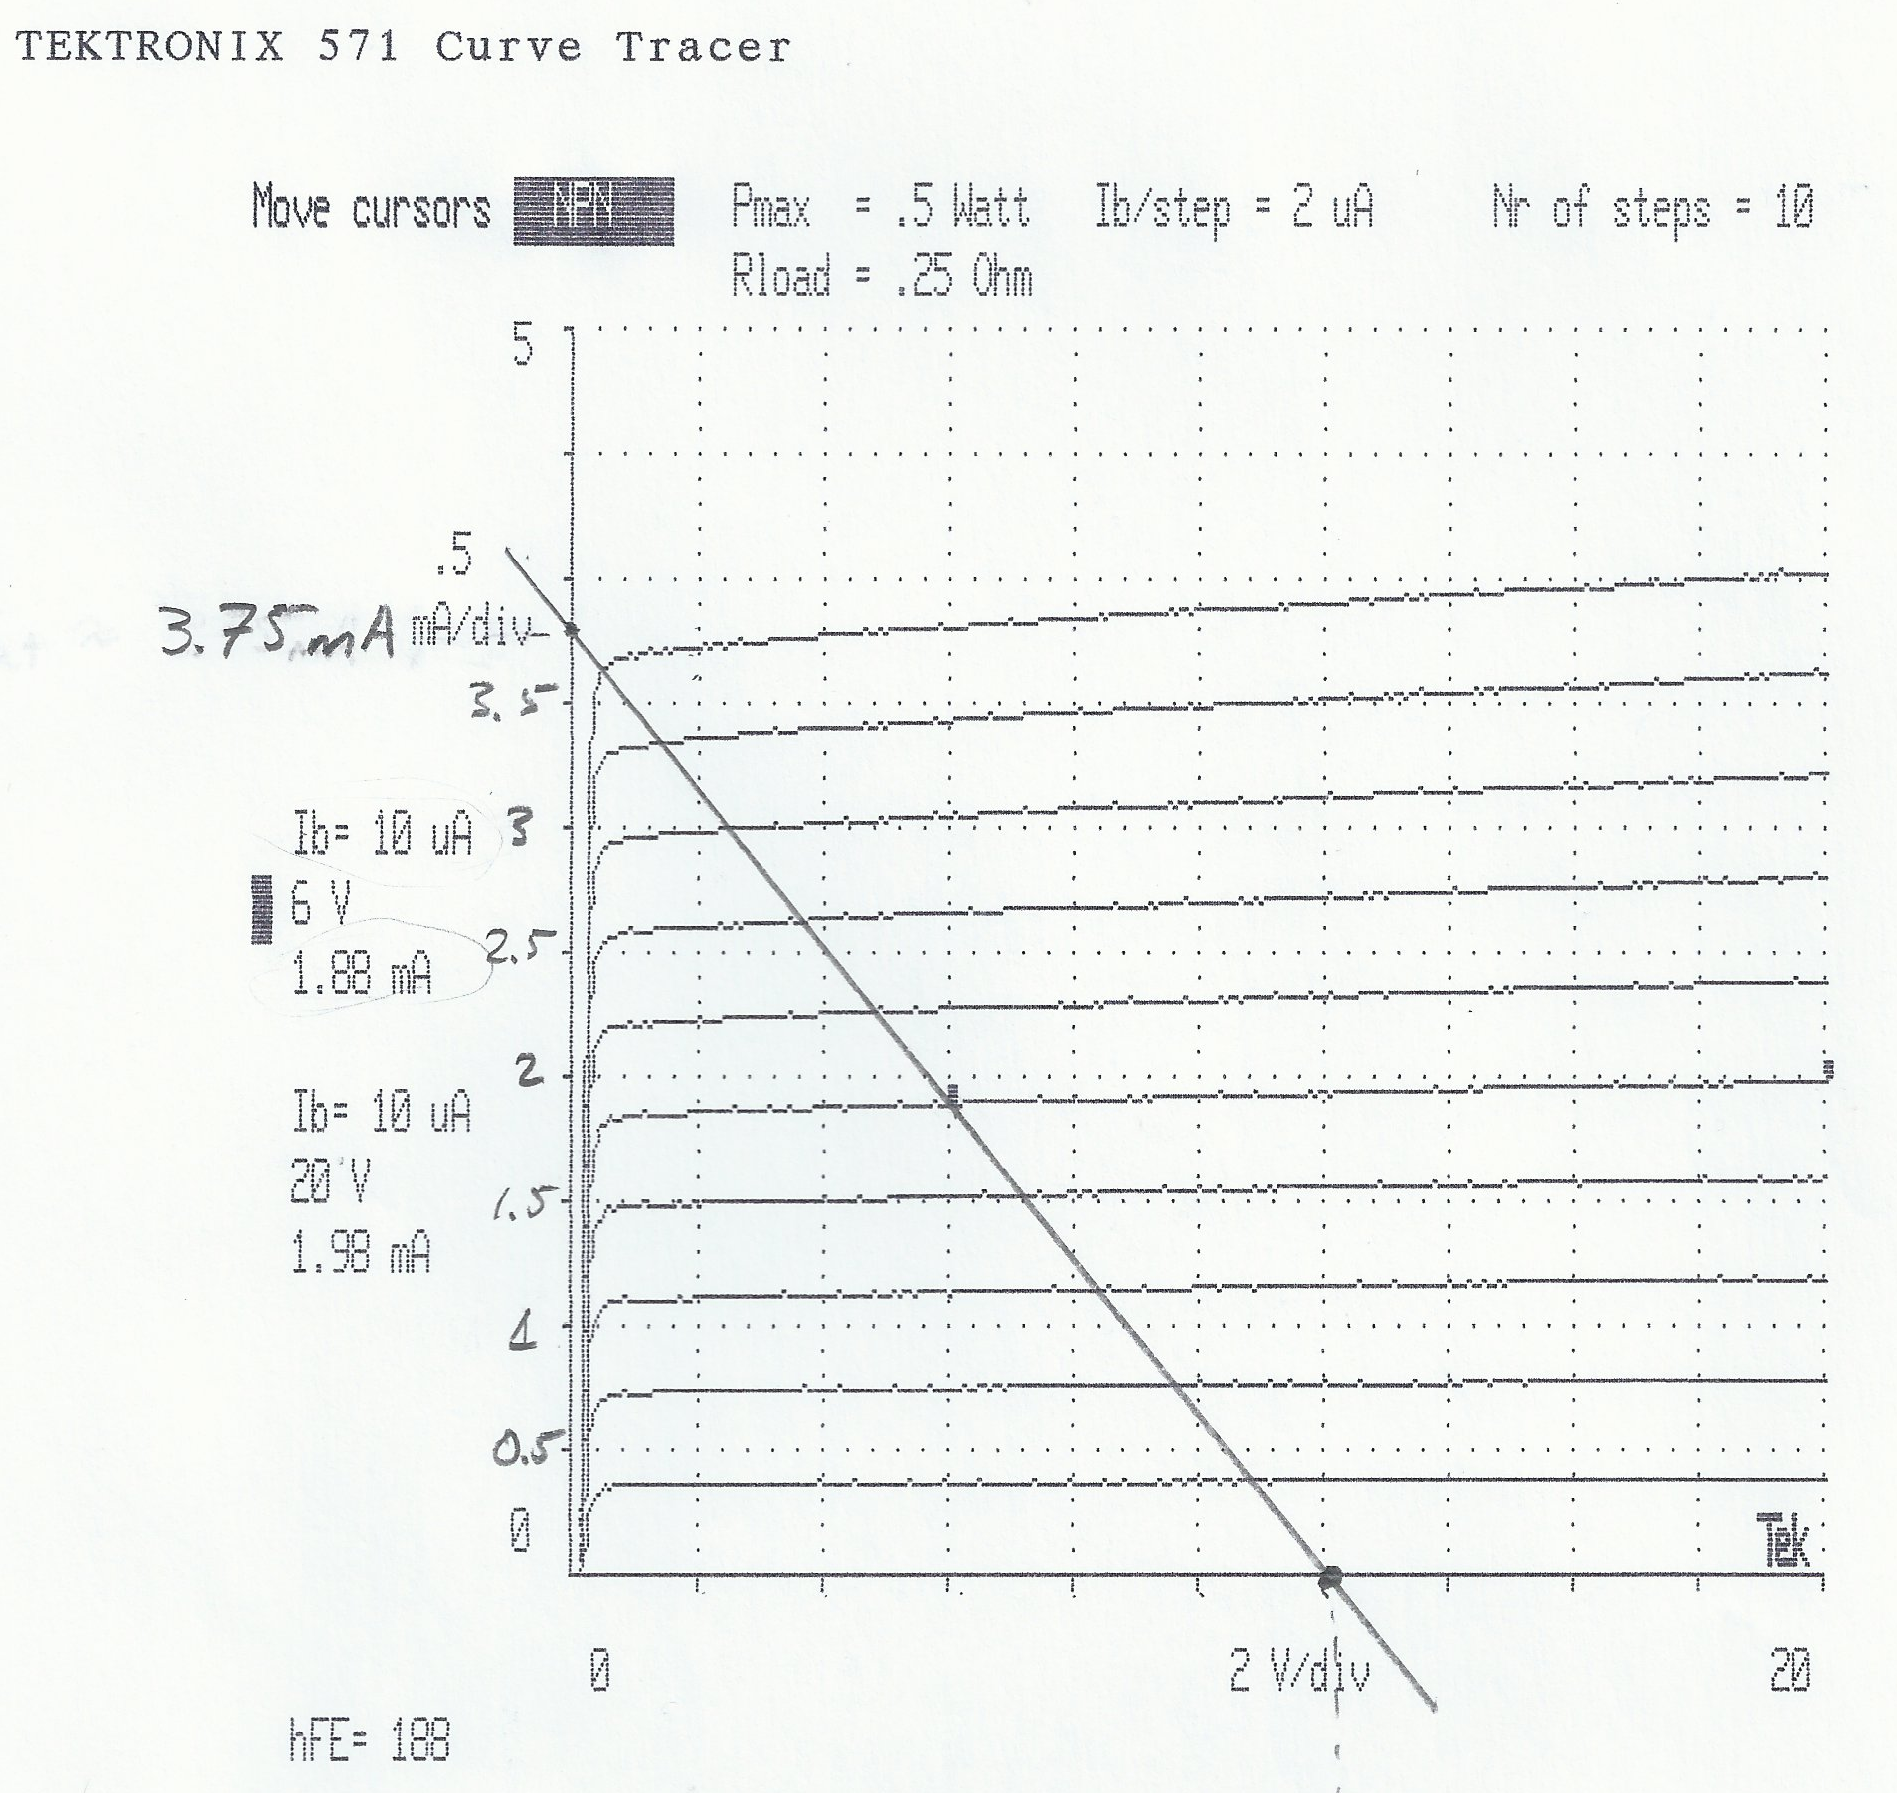
\includegraphics[width=0.6\textwidth]
		{measurements/q2Characteristics}
	\caption{
		Q2 Current-Voltage Characteristics and DC Load Line
	}
	\label{q2Characteristics}
\end{figure}

Putting the desired Q-pt. into equation \ref{ceDCloadEquation}
determined the required emitter resistance.
\begin{equation*}
R_{E2}=\frac{V_{CC}-V_{EE}-V_{CEQ}}{I_{EQ}}=\frac{12V}{1.14mA}
=10.5k\,\Omega
\end{equation*}

The value of $R_{TH}$ should be at least 10 times the emitter
resistance to ensure a stiff base bias. \footnote{A stiff base means
that $R_{1}$ and $R_{2}$ behave like a voltage divider, with 
negligible current being diverted into the base.} Therefore,
\begin{equation*}
R_{TH}=105\,k\Omega=R_{1}||R_{2}
\end{equation*}

If $V_{CEQ}$ is 12V, then the base must be biased at +0.7V to forward
bias the base-emitter junction. The base resistors form a voltage
divider between $V_{CC}$ and $V_{EE}$ to achieve this.
\begin{equation*}
0.7V=\frac{R_{2}}{R_{1}+R_{2}}(24V)-12V
\end{equation*}

Solving the voltage divider equation with the definintion of $R_{TH}$
gives us values for $R_{1}$ and $R_{2}$.
\begin{equation*}
R_{1}=198.4\,k\Omega\qquad\qquad R_{2}=223.0\,k\Omega
\end{equation*}

With DC biasing set, the input resistance of the CE stage is found
from equation \ref{ceRin}.
\begin{equation*}
R_{in2}=(1+\beta)R_{EX}+r_{\pi}=
(1+\beta)(R_{EX}+\nicefrac{V_{th}}{I_{EQ}})
\end{equation*}

The partial bypass resistance is arbitrarily chosen to be
$50\,\Omega$, based on prior experience and the CE voltage gain
(equation \ref{ceAv}). Therefore,
\begin{equation*}
R_{in2}=192(50+\nicefrac{0.0259V}{1.14mA})=14.0\,k\Omega
\end{equation*}

From equation \ref{couplingCapacitors} and using $R_{in2}$,

\begin{equation*}
C_{C2}\geq 11.4\,nF
\end{equation*}

At this point, all of the discrete components for the CB stage have
been determined. A SPICE simulation was performed to check the
performance of the stage. For a load value, the input resistance of
the first common emitter stage was used. The netlist used is included
in appendix \ref{CBstageNetlist} and the results are shown in figure
\ref{CBstageMagnitudePlot}.

\begin{figure}[ht]
	\centering
	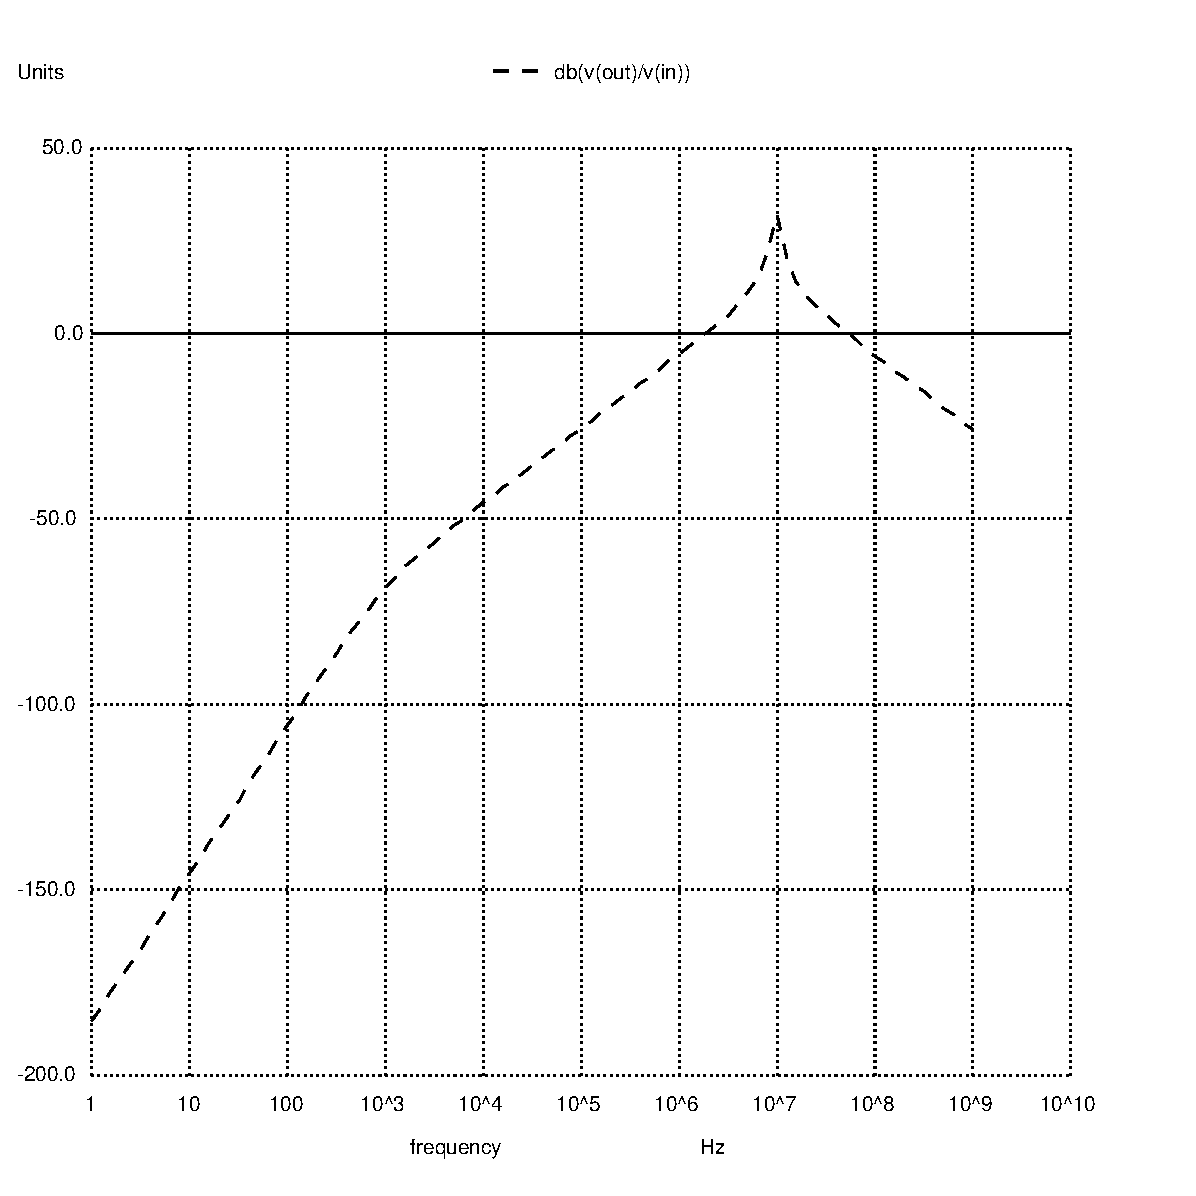
\includegraphics[width=0.6\textwidth]
		{ngspice/CBstage.eps}
	\caption{
		Magnitude Gain of Common-Base Stage, in dB
	}
	\label{CBstageMagnitudePlot}
\end{figure}


\subsection{Common-Emitter Stage III}

Another common-emitter stage was needed to increase the overall
voltage gain. The resistor and capacitor values for this stage were
designed using the same procedure as section \ref{stage2Section}.

The I-V characteristics for Q3 are shown in figure 
\ref{q3Characteristics}.

\begin{figure}[ht]
	\centering
	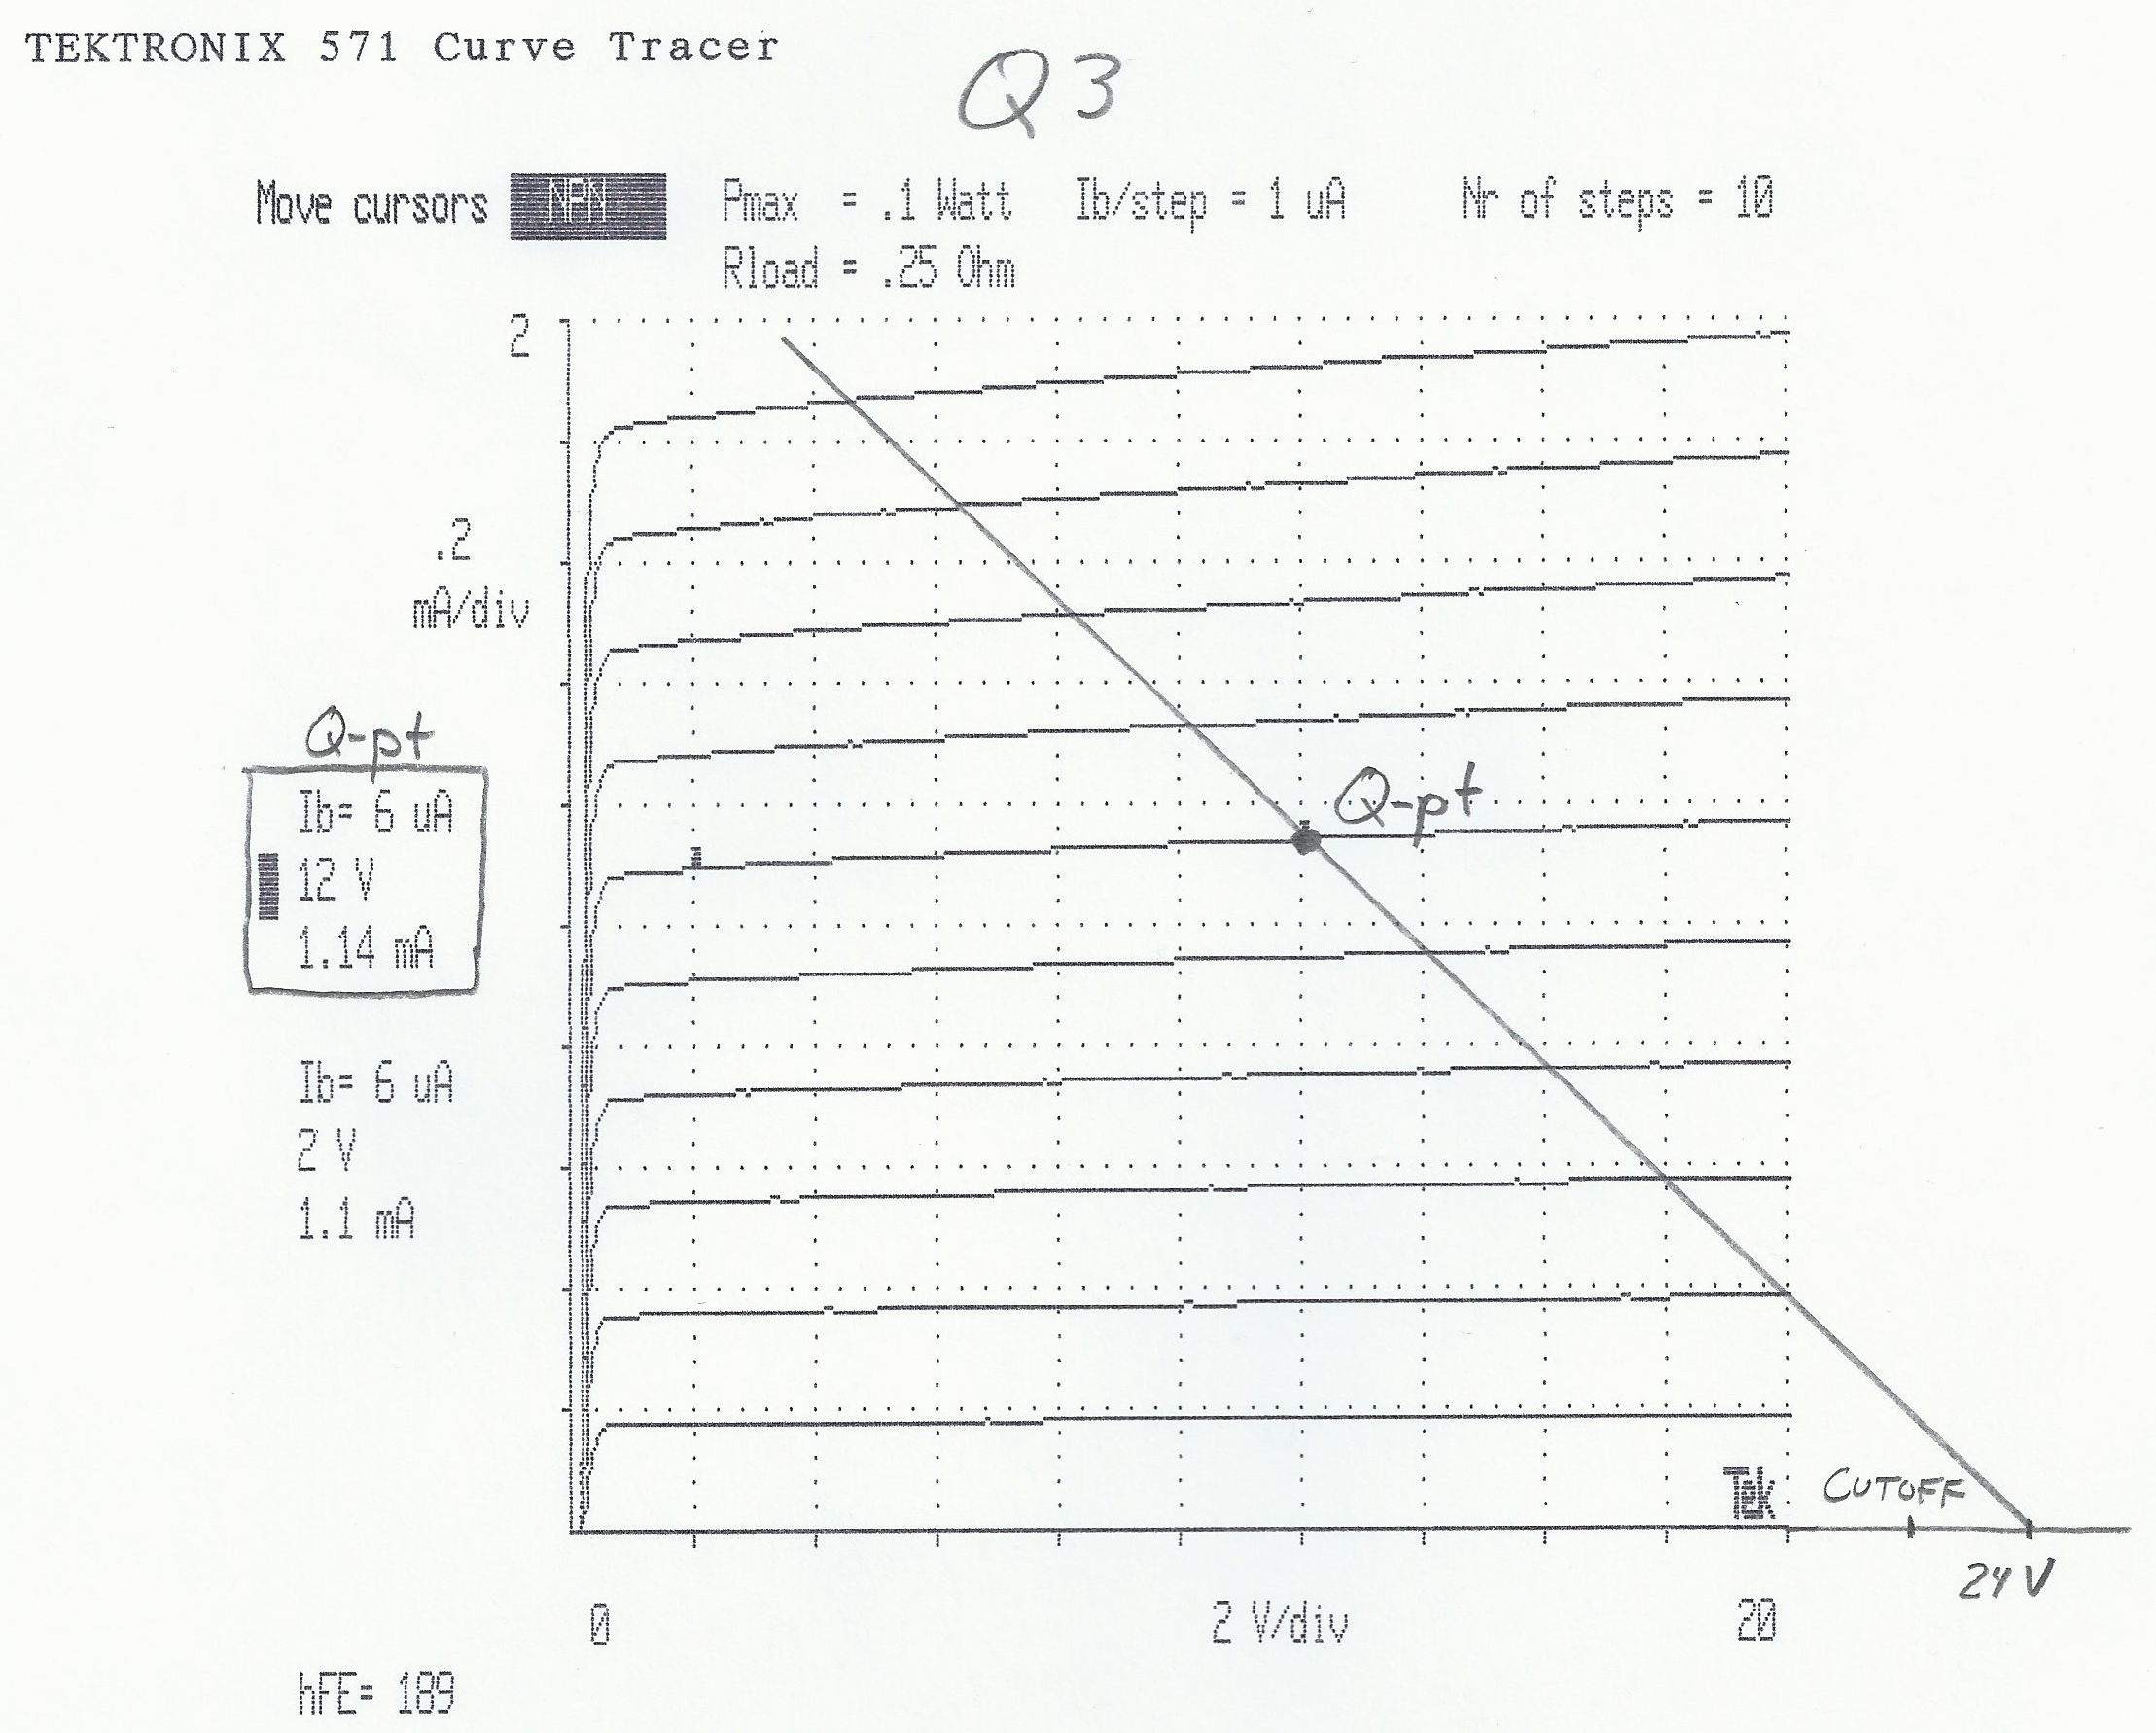
\includegraphics[width=0.6\textwidth]
		{measurements/q3Characteristics}
	\caption{
		Q3 Current-Voltage Characteristics and DC Load Line
	}
	\label{q3Characteristics}
\end{figure}

Astonishingly conveniently
\footnote{or perhaps astonishingly cleverly},
the Q-pt curser for Q3 was identical to Q2. Therefore, the discrete
resistors and capacitors needed for stage 3 are the same as stage 2.

\subsection{Common-Collector Stage IV}

The Q-pt. of the common-collector stage must be chosen to achieve the
specified output impedance of 50 ohms. The relationship between the
two was found in equation \ref{ccRo}.
\begin{equation*}
50\,\Omega=R_{o}=\frac{V_{th}}{I_{EQ}}
\qquad\rightarrow\qquad I_{EQ(Q4)}=5.2\,mA
\end{equation*}

The quiescent collector-emitter voltage is chosen to be 12 V to split
the power supplies evenly. Ohms law is used to calculate an emitter
resistance that will limit $I_{EQ}$ given a potential difference of
12 V.
\begin{equation*}
R_{E4}=\frac{V_{CC}-V_{EE}-V_{CEQ}}{I_{EQ}}=23.2k\,\Omega
\end{equation*}

There is not really a point in plotting a load line because the load
on the collector is zero. Nevertheless, it has been plotted on the
I-V characteristics shown in figure \ref{q4Characteristics}.

\begin{figure}[ht]
	\centering
	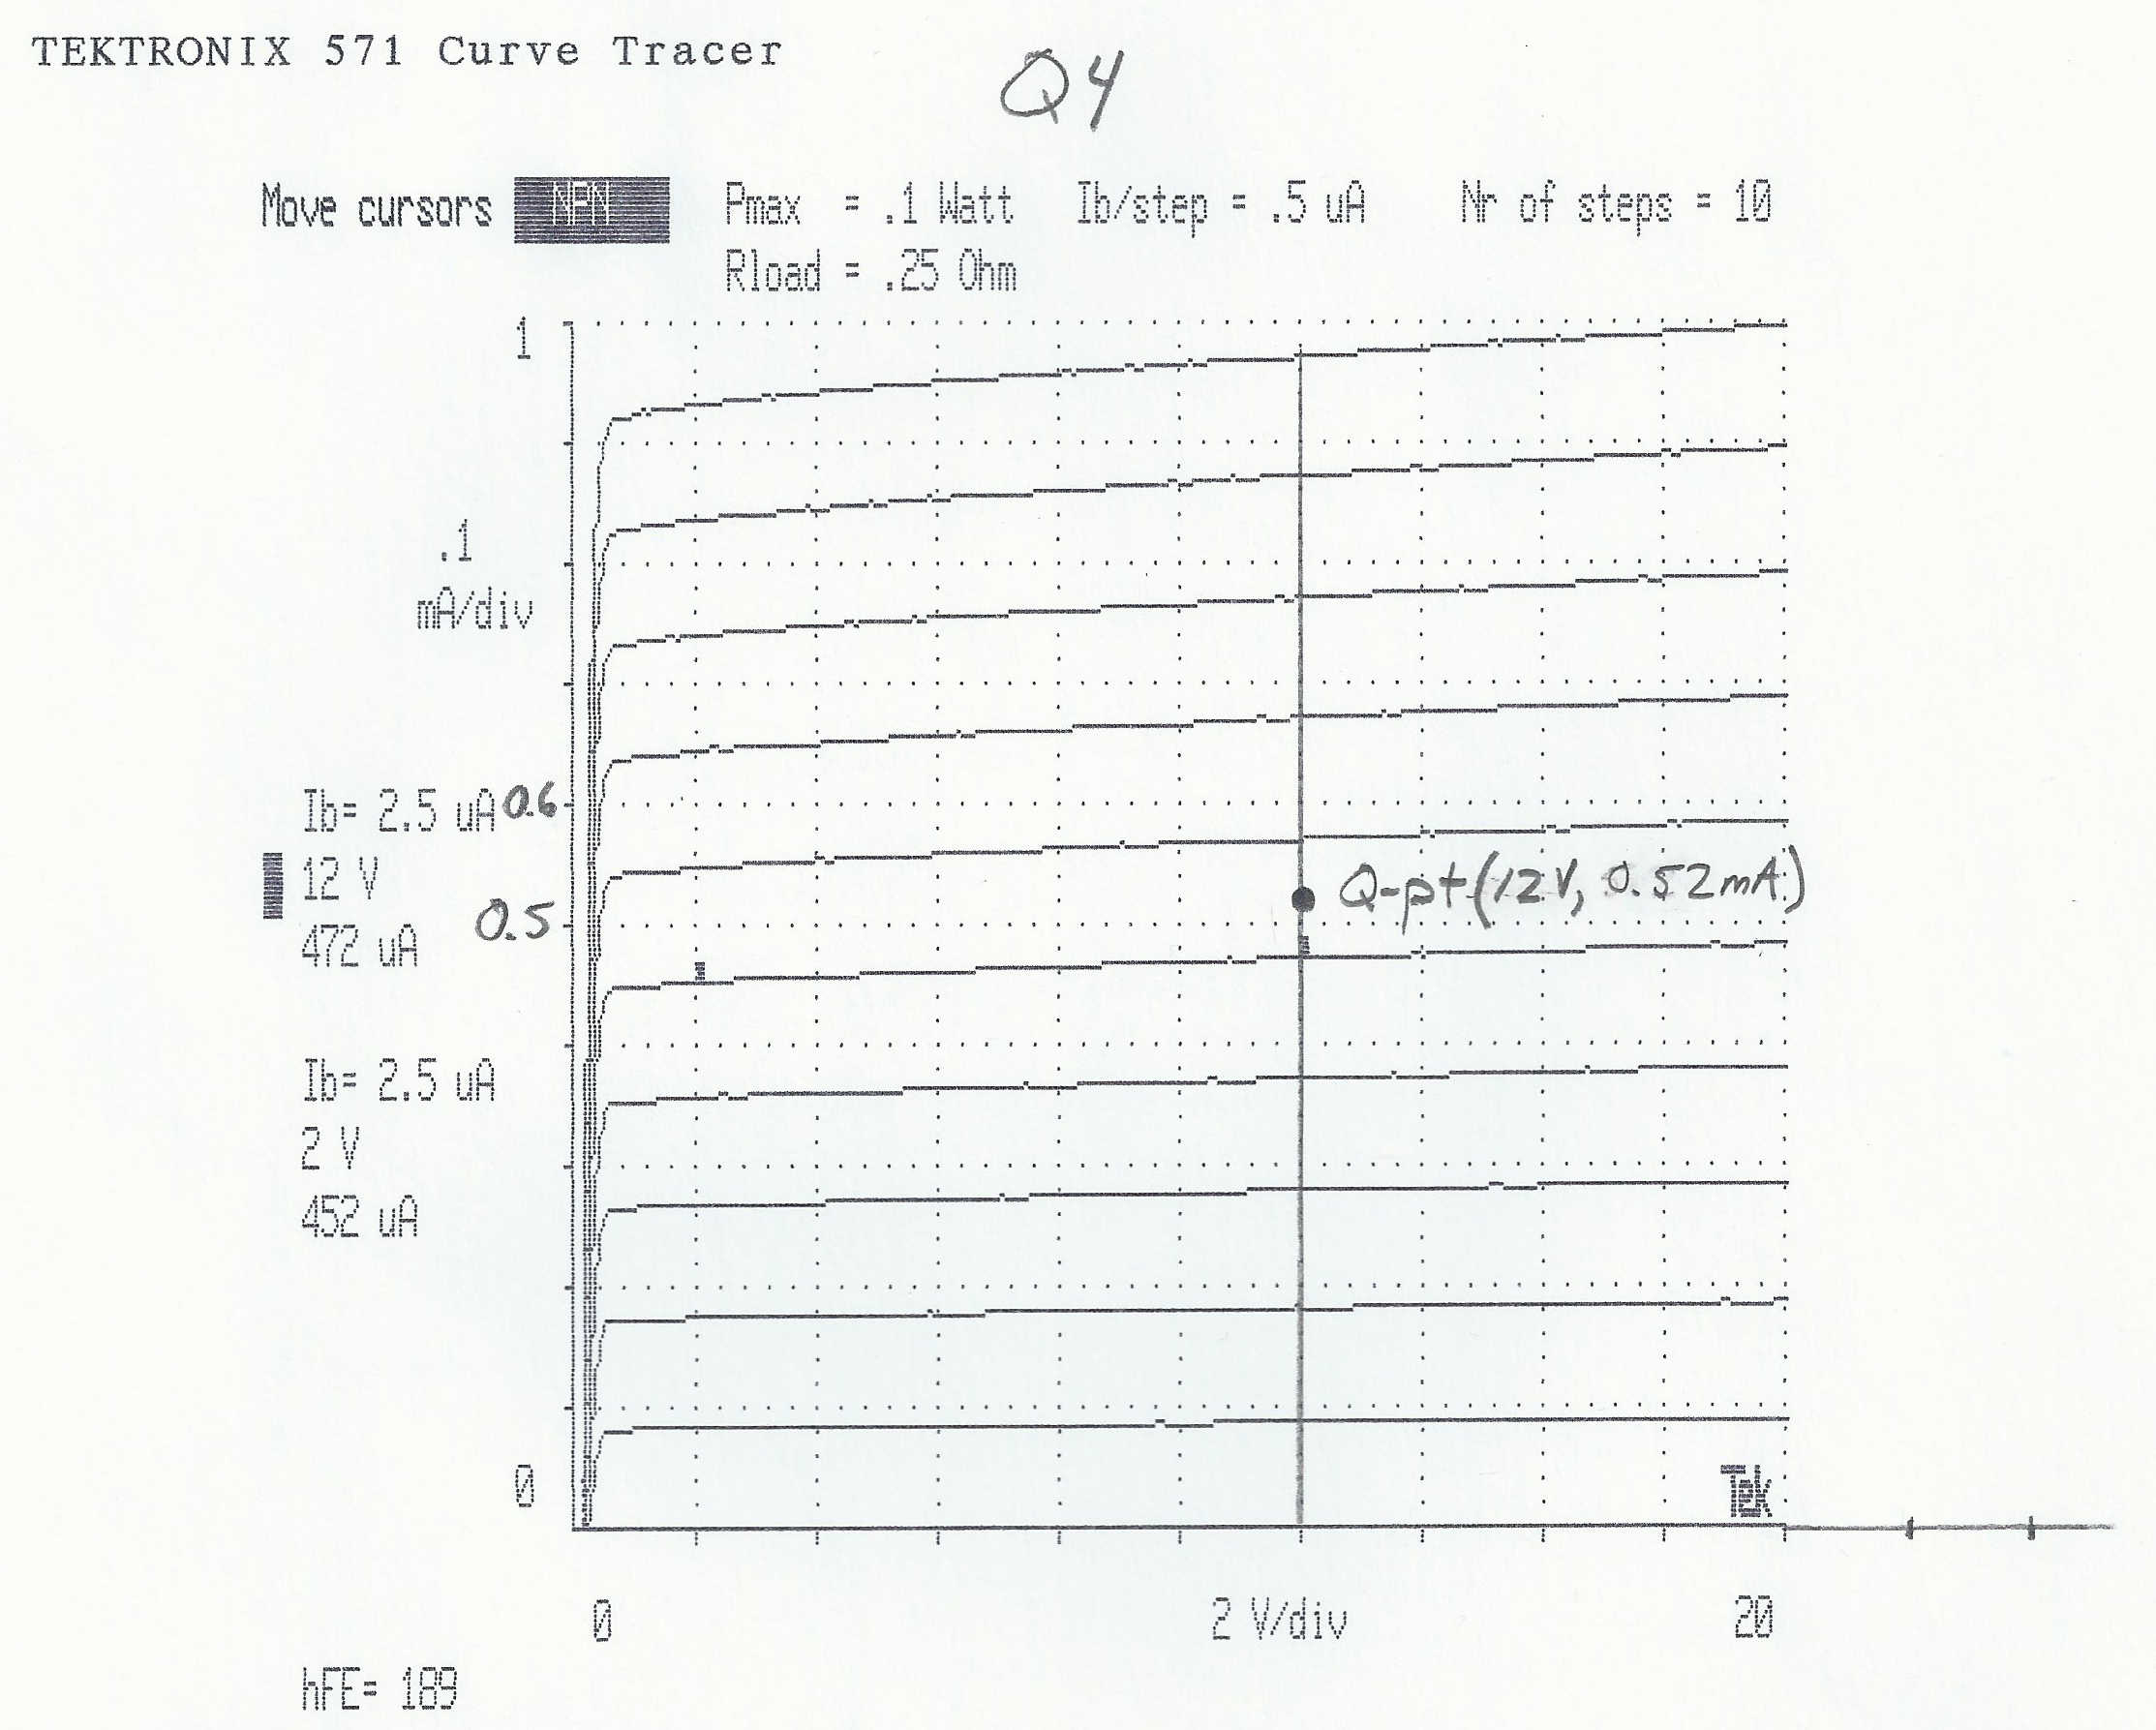
\includegraphics[width=0.6\textwidth]
		{measurements/q4Characteristics}
	\caption{
		Q4 Current-Voltage Characteristics and DC Load Line
	}
	\label{q4Characteristics}
\end{figure}

To hold a stiffly biased base at 0.7 V, the thevenin equivalent
resistance should be $\nicefrac{1}{10}$ the reflected base-emitter
resistance.
\begin{equation*}
R_{TH}=0.1(\beta+1)R_{E}=0.1(190)(23.2k)=440.8\,k\Omega
\end{equation*}

Solving the thevenin resistance equation and a voltage divider for
+0.7 volts simultaneously designates values for $R_{5}$ and $R_{6}$.
\begin{equation*}
R_{5}=833\,k\Omega\qquad\textrm{and}\qquad R_{6}=936.2\,k\Omega
\end{equation*}

It is probably safe to copy coupling capacitor values from elsewhere
in the circuit. The output coupling should be identical to the input
coupling because they are both look out on as little as 50 ohms external
impedance.
\begin{equation*}
C_{c4}=11.4nF\qquad\textrm{and}\qquad C_{c5}=C_{c1}=3.18\,\mu F
\end{equation*}

\section{Appendices}

\subsection{HP 4342A Q Meter}
\label{qMeter}

The following 3 pages are taken from the HP 4342A Q Meter Operating
and Service Manual, pages 35-37.

\clearpage
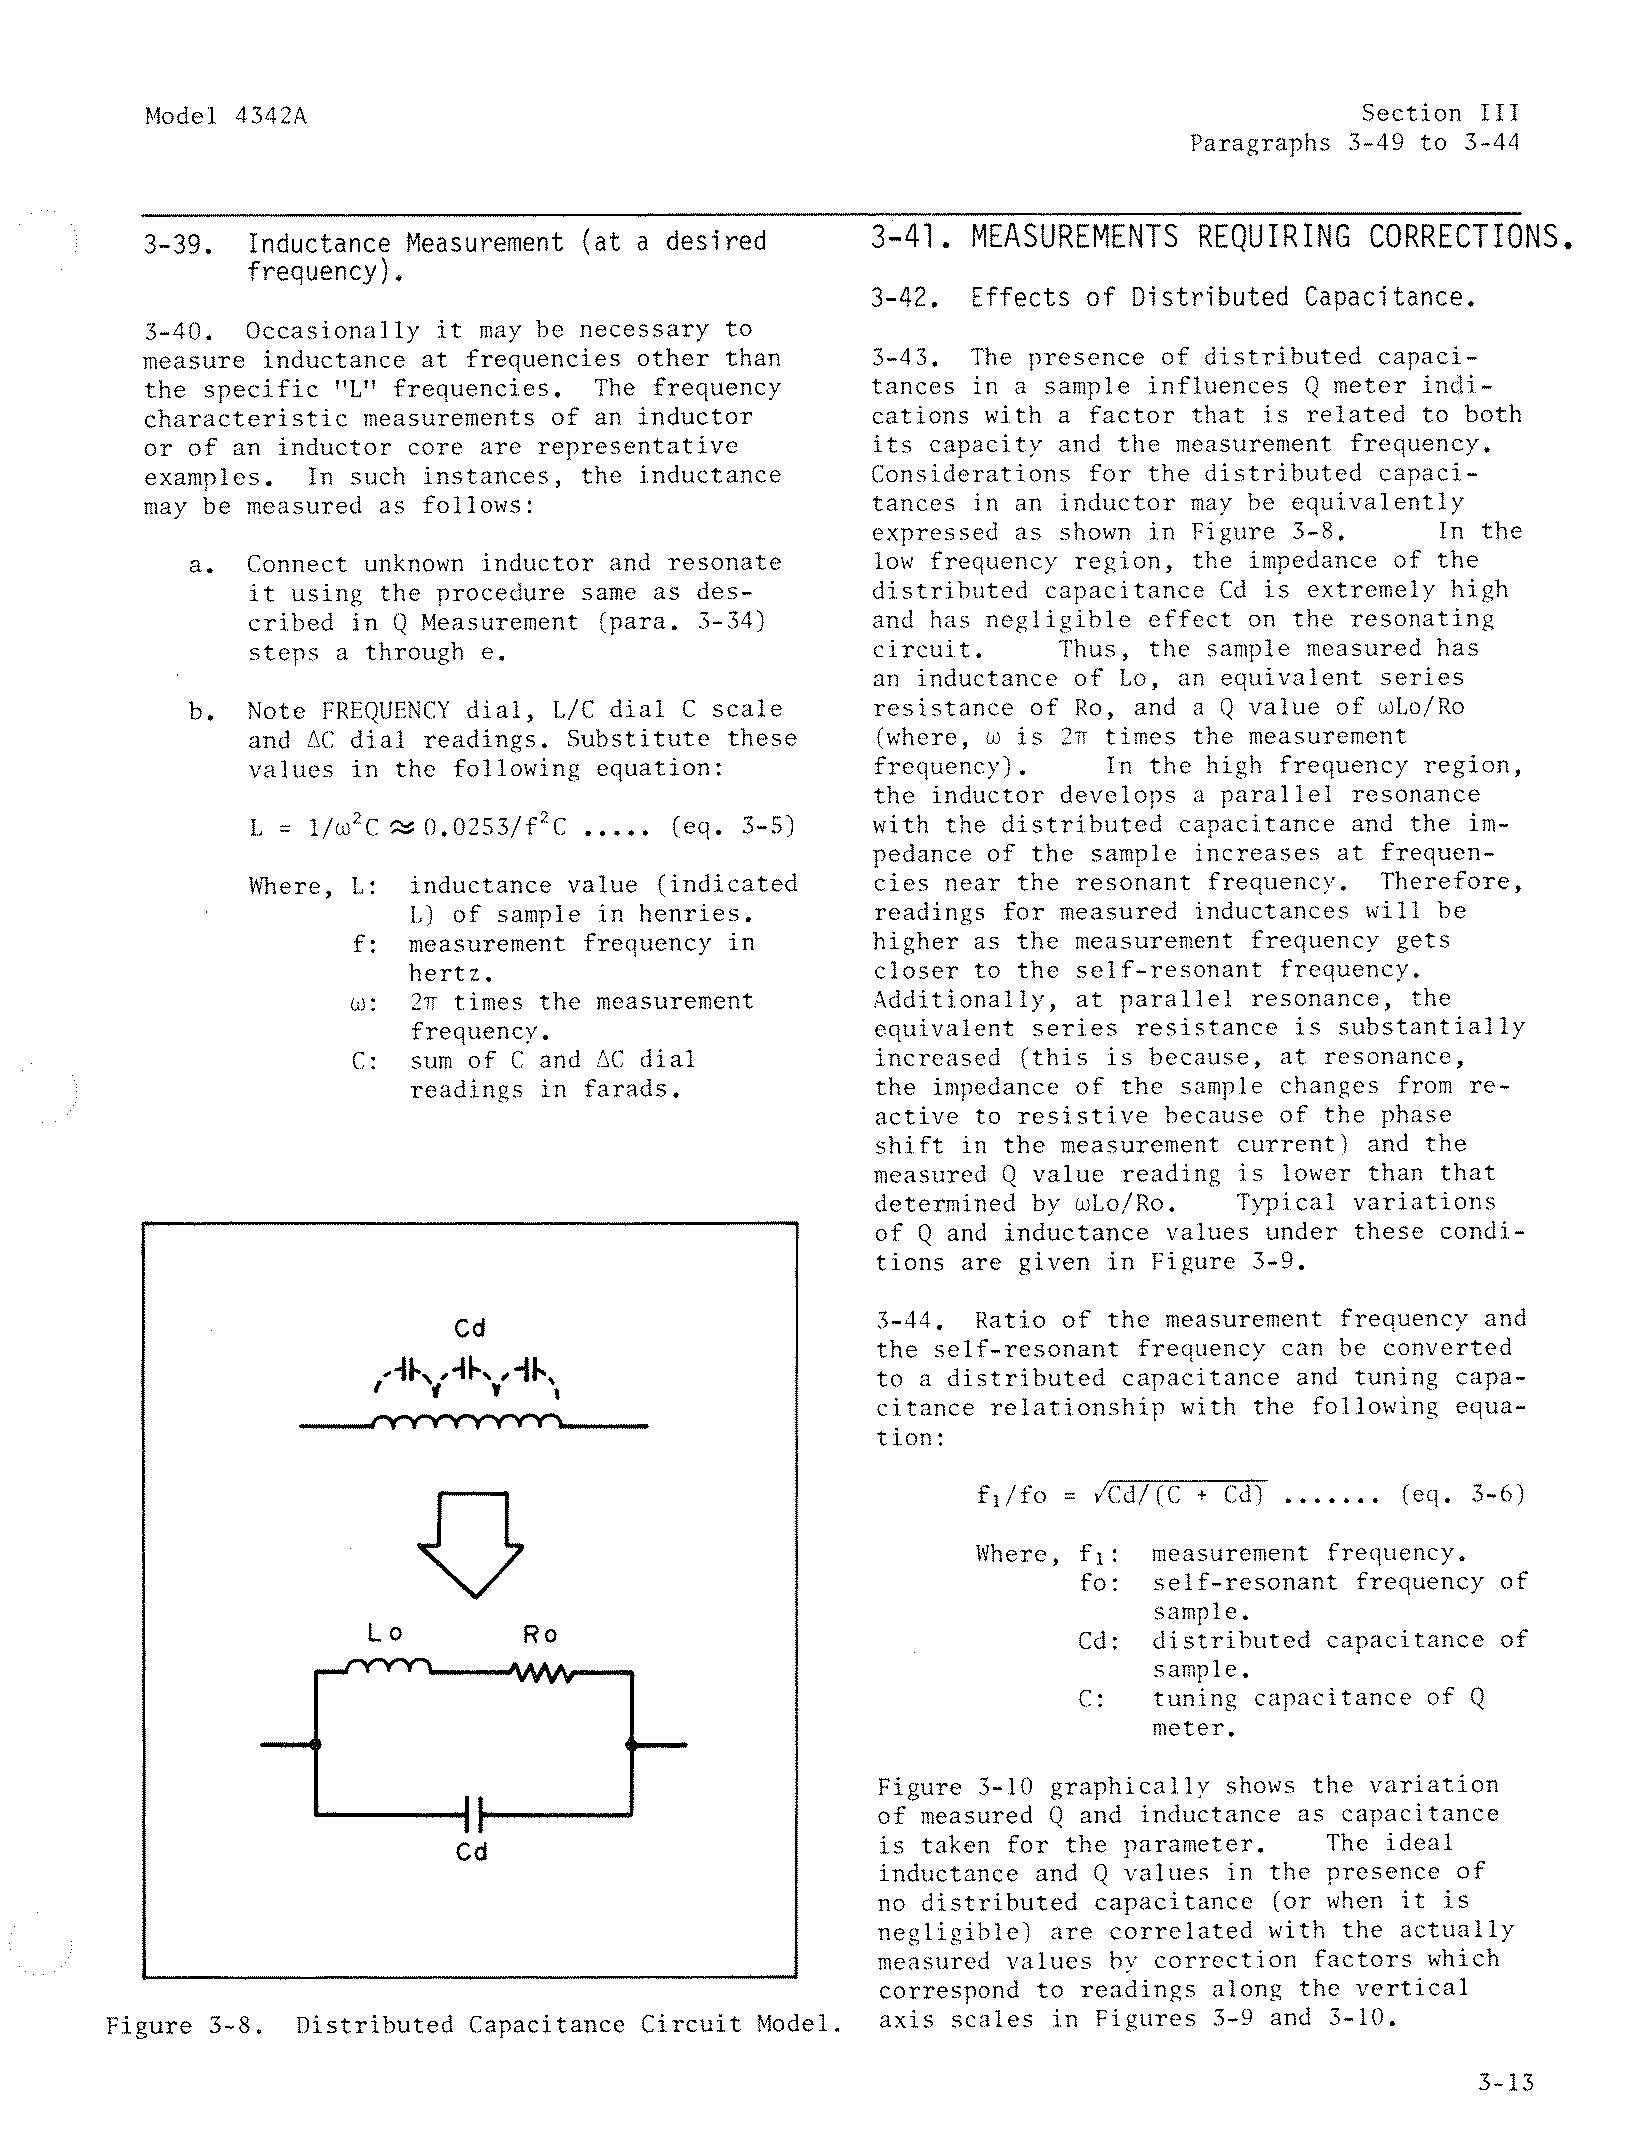
\includegraphics[width=1\textwidth]{qMeter/page35}

\pagebreak
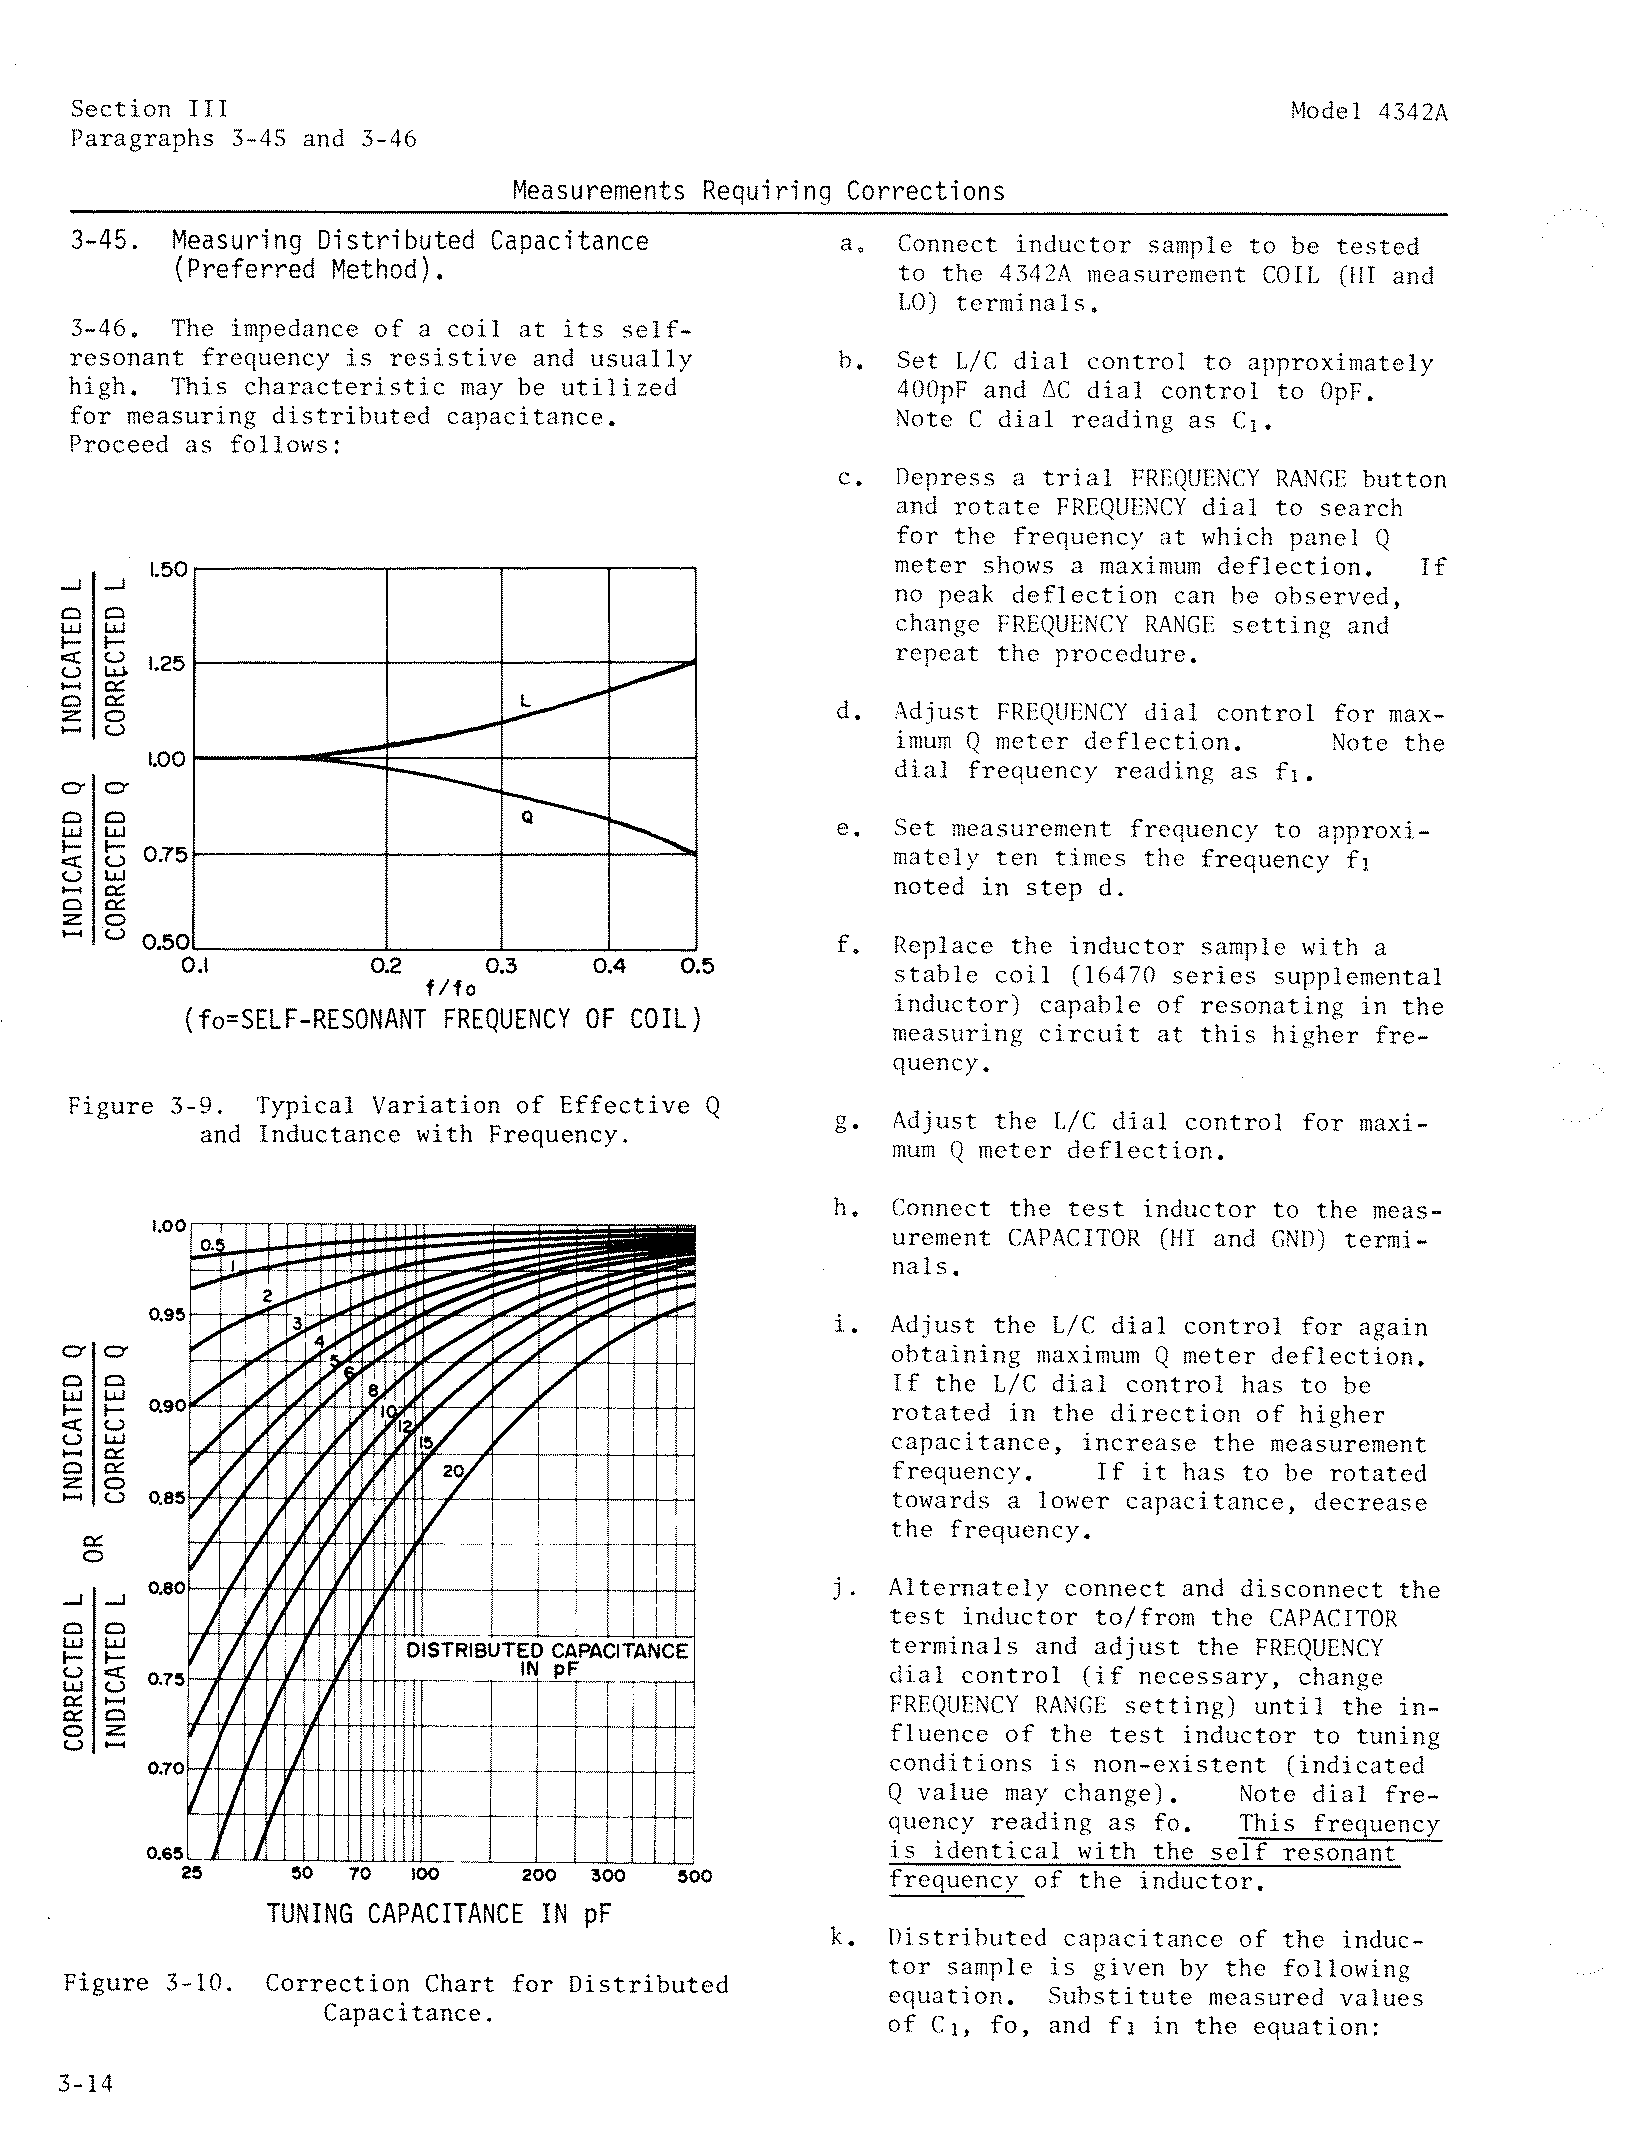
\includegraphics[width=1\textwidth]{qMeter/page36}

\pagebreak
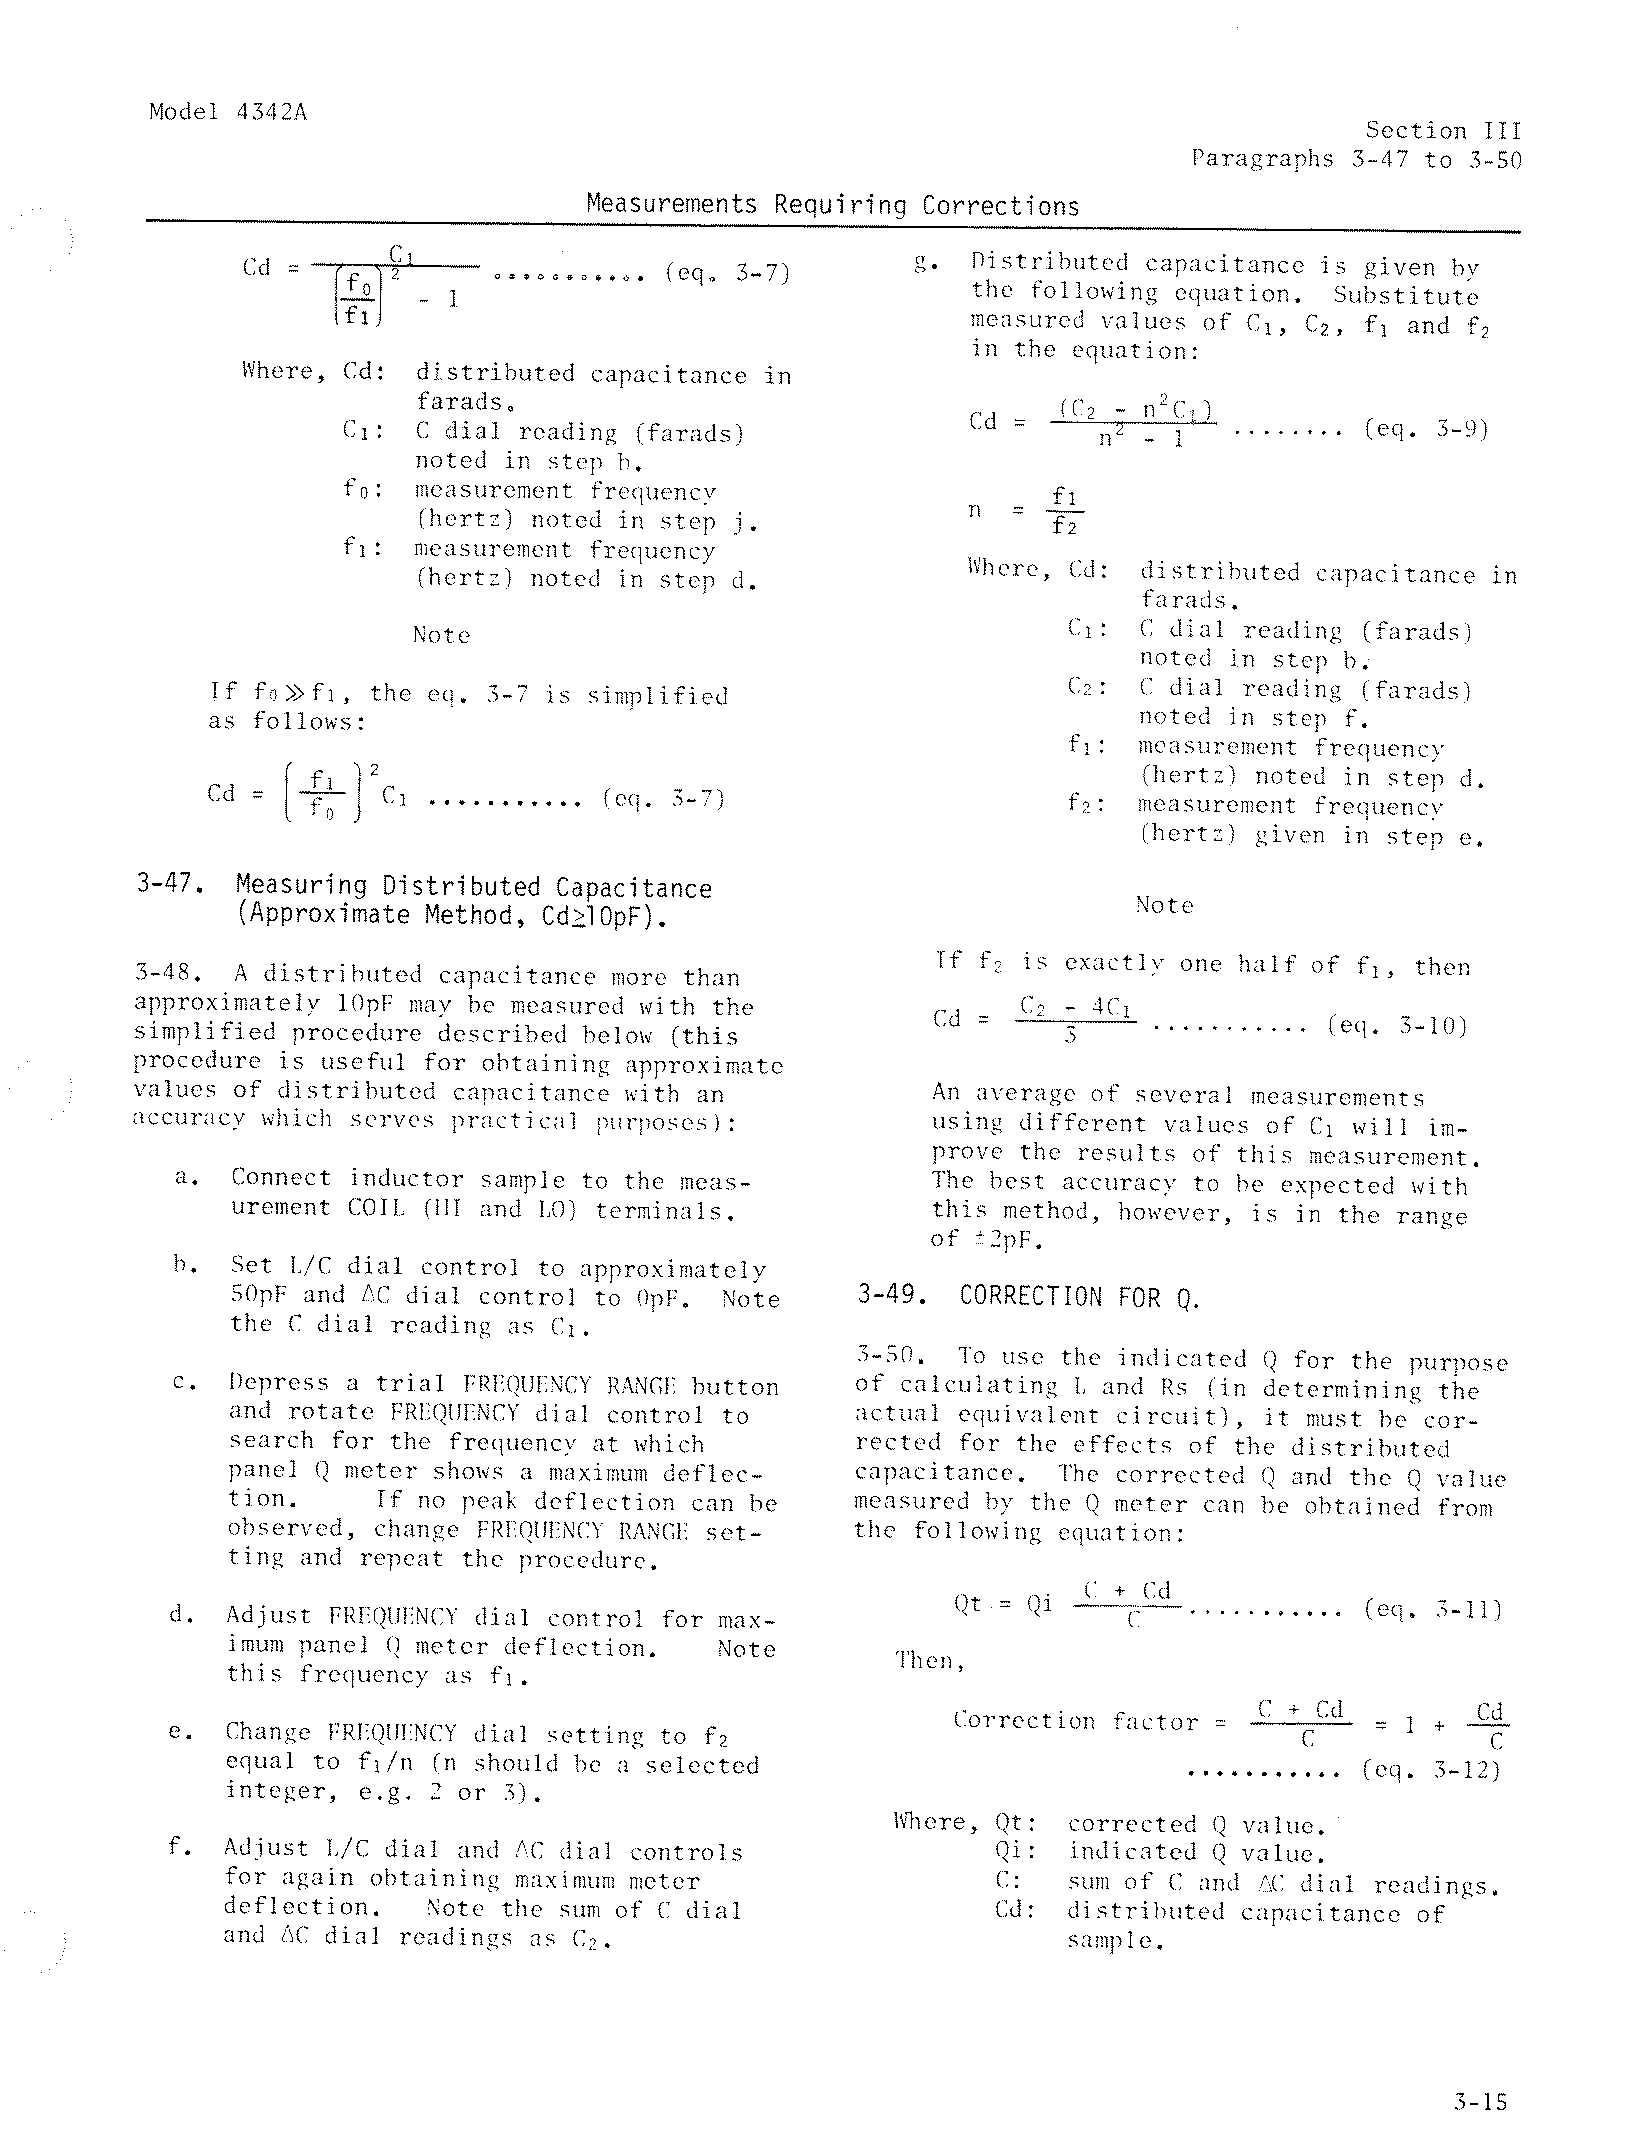
\includegraphics[width=1\textwidth]{qMeter/page37}

\pagebreak
\subsection{Common-Base SPICE Netlist}
\label{CBstageNetlist}

The following netlist was used to simulate the CB stage. The labeling
in the netlist corresponds to the circuit in figure
\ref{commonBaseStage}.

\begin{verbatim}
*** CBstage.cir ***
* Nodes:
* gnd, cc (+12V), ee (-12V), s, in, e1, c1, out

Vcc cc gnd dc 12V ac 0V
Vee ee gnd dc -12V ac 0V
Vs s gnd dc 0V ac 10mV
Rs in s 50
Cc1 in e1 3.183uF
Re1 e1 ee 21.8k
Q1 c1 gnd e1 model1
L1 c1 cc 4.2uH
Cd1 c1 cc 55pF
Rp1 c1 cc 2.18k
Cc2 c1 out 3.183uF
Rld out gnd 9999k

* .model <name> <type> (par1=value1 par2=value2 ...)
* VAF = forward Early voltage
* BF = forward beta; forward common-emitter gain
* CJE = base-emitter zero-bias junction capacitance
* CJC = base-collector zero-bias junction capacitance
* TS = transport saturation current
* NF = forward mode ideality factor

.model model1 npn (BF=176 CJC=20pf CJE=20pf IS=1E-16 VAF=452V NF=1)

.control
set filetype=ascii
ac dec 10 1Hz 1GHz
plot db(v(out)/v(in))
plot ph(v(out))-ph(v(in))
write CBstage.txt db(v(output)/v(input)) ph(v(output))-ph(v(input))
\end{verbatim}

\subsection{MATLAB Script for $A_{v}(I_{EQ})$}
\label{matlabScript}

\begin{verbatim}
PUT CODE HERE!
\end{verbatim}

\end{document}
